\documentclass[11pt,oneside,letterpaper]{article}

% graphicx package, useful for including eps and pdf graphics
\usepackage{graphicx}
\DeclareGraphicsExtensions{.png,.png,.jpg}

% basic packages
\usepackage{color}
\usepackage{parskip}
\usepackage{float}
\usepackage{microtype}
\usepackage{url}
\usepackage{hyperref}

% text layout
\usepackage{geometry}
\geometry{textwidth=17cm} % 15.25cm for single-space, 16.25cm for double-space
\geometry{textheight=22.5cm} % 22cm for single-space, 22.5cm for double-space

% helps to keep figures from being orphaned on a page by themselves
\renewcommand{\topfraction}{0.85}
\renewcommand{\textfraction}{0.1}

% bold the 'Figure #' in the caption and separate it with a period
% Captions will be left justified
\usepackage[labelfont=bf,labelsep=period,font=small]{caption}

% review layout with double-spacing
%\usepackage{setspace}
%\doublespacing
%\captionsetup{labelfont=bf,labelsep=period,font=doublespacing}

% cite package, to clean up citations in the main text. Do not remove.
\usepackage{cite}
%\renewcommand\citeleft{(}
%\renewcommand\citeright{)}
%\renewcommand\citeform[1]{\textsl{#1}}

% Remove brackets from numbering in list of References
\renewcommand\refname{\large References}
\makeatletter
\renewcommand{\@biblabel}[1]{\quad#1.}
\newcommand{\FIG}[1]{Fig.~\ref{#1}}
\makeatother

\usepackage{authblk}
\renewcommand\Authands{ \& }
\renewcommand\Authfont{\normalsize \bf}
\renewcommand\Affilfont{\small \normalfont}
\makeatletter
\renewcommand\AB@affilsepx{, \protect\Affilfont}
\makeatother

%%% TOC
\usepackage{patchcmd}
\makeatletter
\patchcommand\@starttoc{\begin{quote}}{\end{quote}}
\usepackage{tocloft}
\renewcommand{\cftsecleader}{\cftdotfill{\cftdotsep}}

%%% TITLE %%%
\title{\vspace{2cm} \LARGE \bf
Seasonal influenza circulation patterns and projections for 2017-2018
}

\author[1]{Trevor Bedford}
\author[2]{Richard A.\ Neher}

\affil[1]{Vaccine and Infectious Disease Division, Fred Hutchinson Cancer Research Center, Seattle, WA, USA}
\affil[2]{Biozentrum, University of Basel, Basel, Switzerland}

\date{September 15, 2017}
\begin{document}

\maketitle

\emph{This is not meant as a comprehensive report, but is instead
intended as particular observations that we've made that may be of
relevance. Please also note that observed patterns reflect the GISAID
database and may not be entirely representative of underlying dynamics.}

\tableofcontents

\pagebreak
\section*{A/H3N2}
\addcontentsline{toc}{section}{A/H3N2}

\textbf{H3N2 continues to diversify with many coexisting clades, all of
which carry several amino acid mutations at previously characterized
epitopes. The majority of viruses fall into the 3c2.a clade which has
been dominating globally for \textgreater{}3 years, but 3c3.a viruses
continue to persist. The common ancestor of circulating H3N2 viruses is
now more than 5 years old, which is rare for H3N2. Despite extensive
genetic diversity, serological assays suggest limited, but non-zero,
antigenic evolution. We expect multiple competing clades within 3c2.a to
persist into the future with no clear immediate winner.}

We base our primary analysis on a set of viruses collected between Oct
2015 and Aug 2017, comprising \textgreater{}800 viruses per month in Dec
2016 to Mar 2017 and 100-200 viruses per month more recently, see \FIG{H3N2_counts}. We use all
available data when estimating frequencies of mutations and weight
samples appropriately by regional population size and relative sampling
intensity to arrive at a putatively unbiased global frequency estimate.
Phylogenetic analyses are based on a representative sample of about 2000
viruses.

\begin{figure}[H]
  \centering
  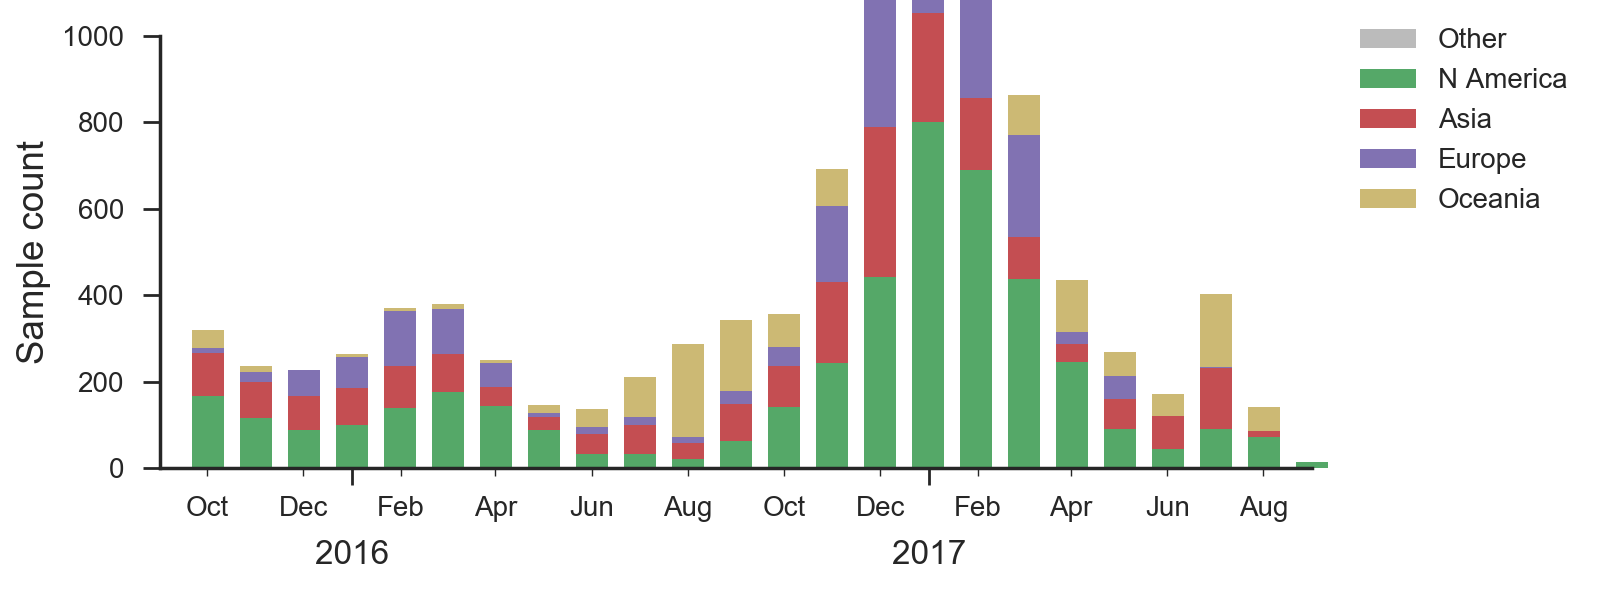
\includegraphics[width=0.9\textwidth]{../figures/sep-2017/h3n2_counts.png}
  \caption{\textbf{Sample counts through time and across regions.}
  This is a stacked bar plot, so that in all months there are at least 100 samples, in some month $>500$ sequences.
  }
  \label{H3N2_counts}
\end{figure}

\clearpage
\begin{figure}[H]
  \centering
  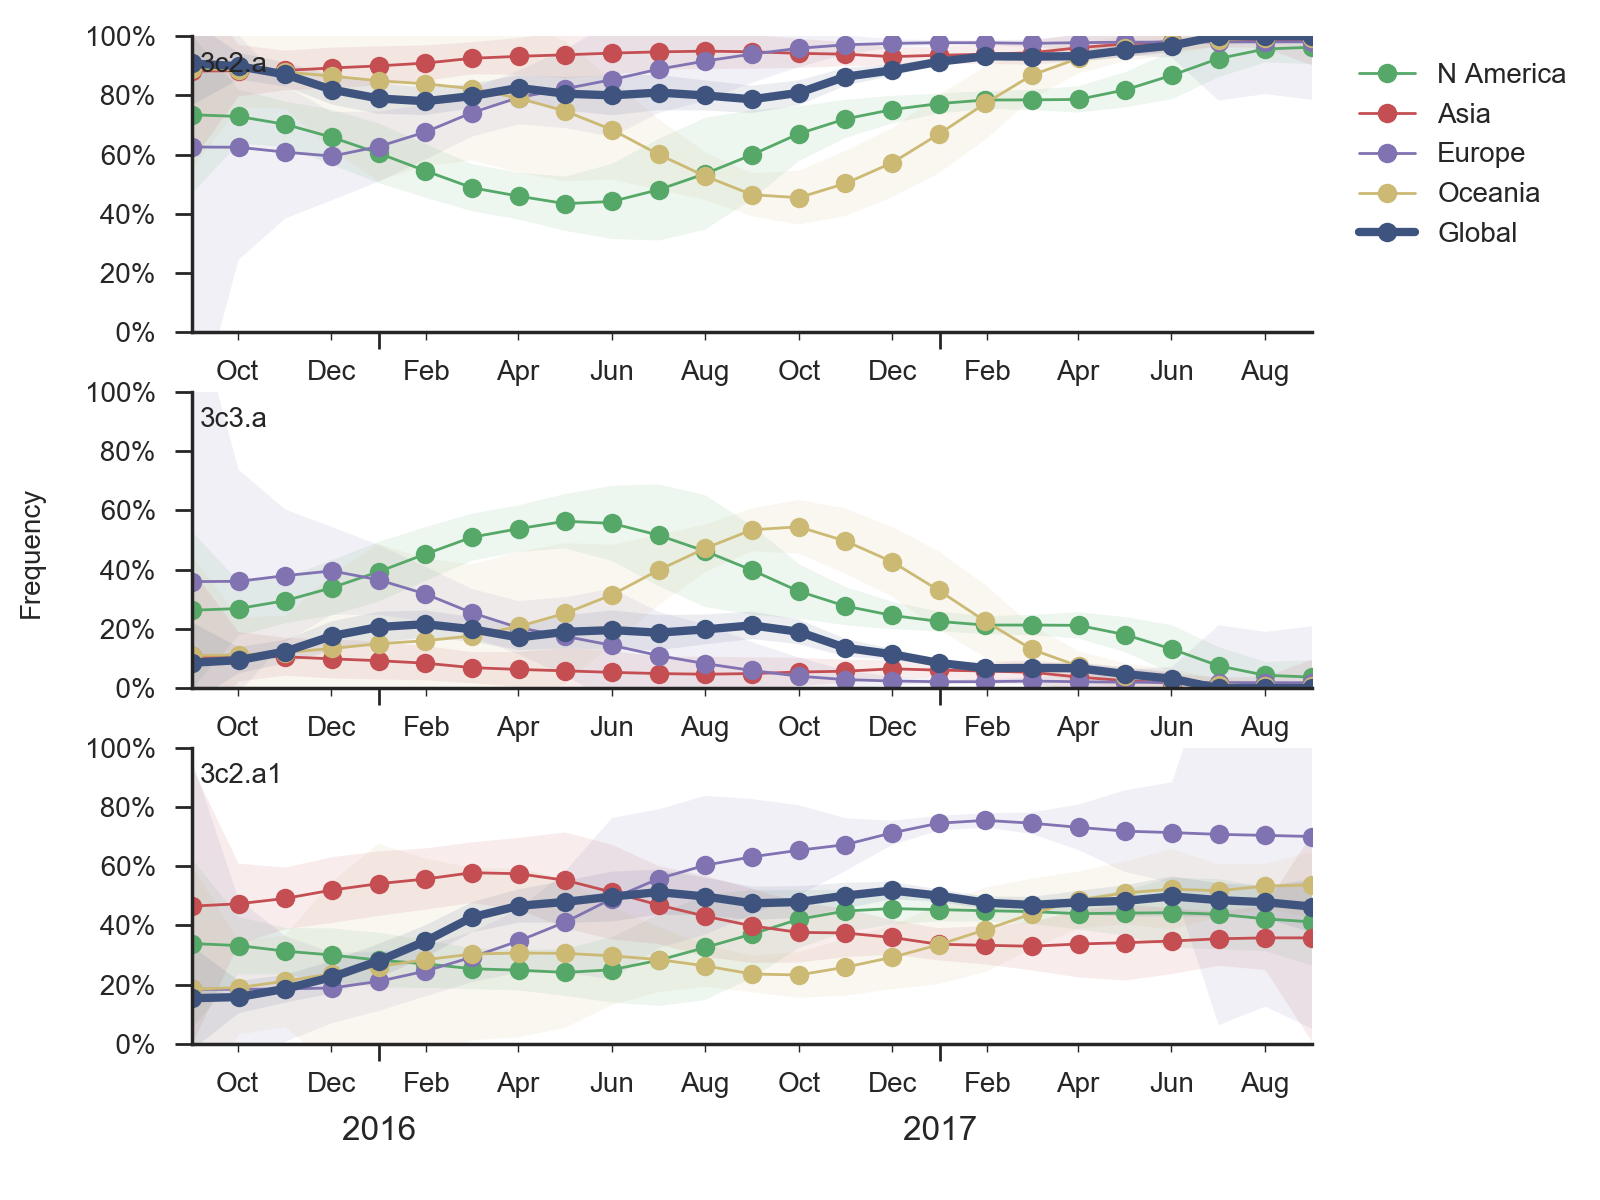
\includegraphics[width=0.9\textwidth]{../figures/sep-2017/h3n2_clades.png}
  \caption{\textbf{Dynamics of major H3N2 clades.} Clade 3c3.a continues to circulate at low frequency, while 3c3.b has not been observed for several month (not shown).}
  \label{H3N2_clades}
\end{figure}
At the level of major clades, 3c2.a has continued to dominate while
3c3.a persisted at about 20\% frequency in Oceania and North America in
the 2016-2017 season, see \FIG{H3N2_clades}. Within 3c2.a, the clade 3c2.a1 comprising HA1
mutation N171K and HA2 mutations I77V and G155E had risen rapidly in
early 2016 but later stabilized at about 50\% with somewhat higher
frequencies in Europe.

\clearpage
\begin{figure}[H]
  \centering
  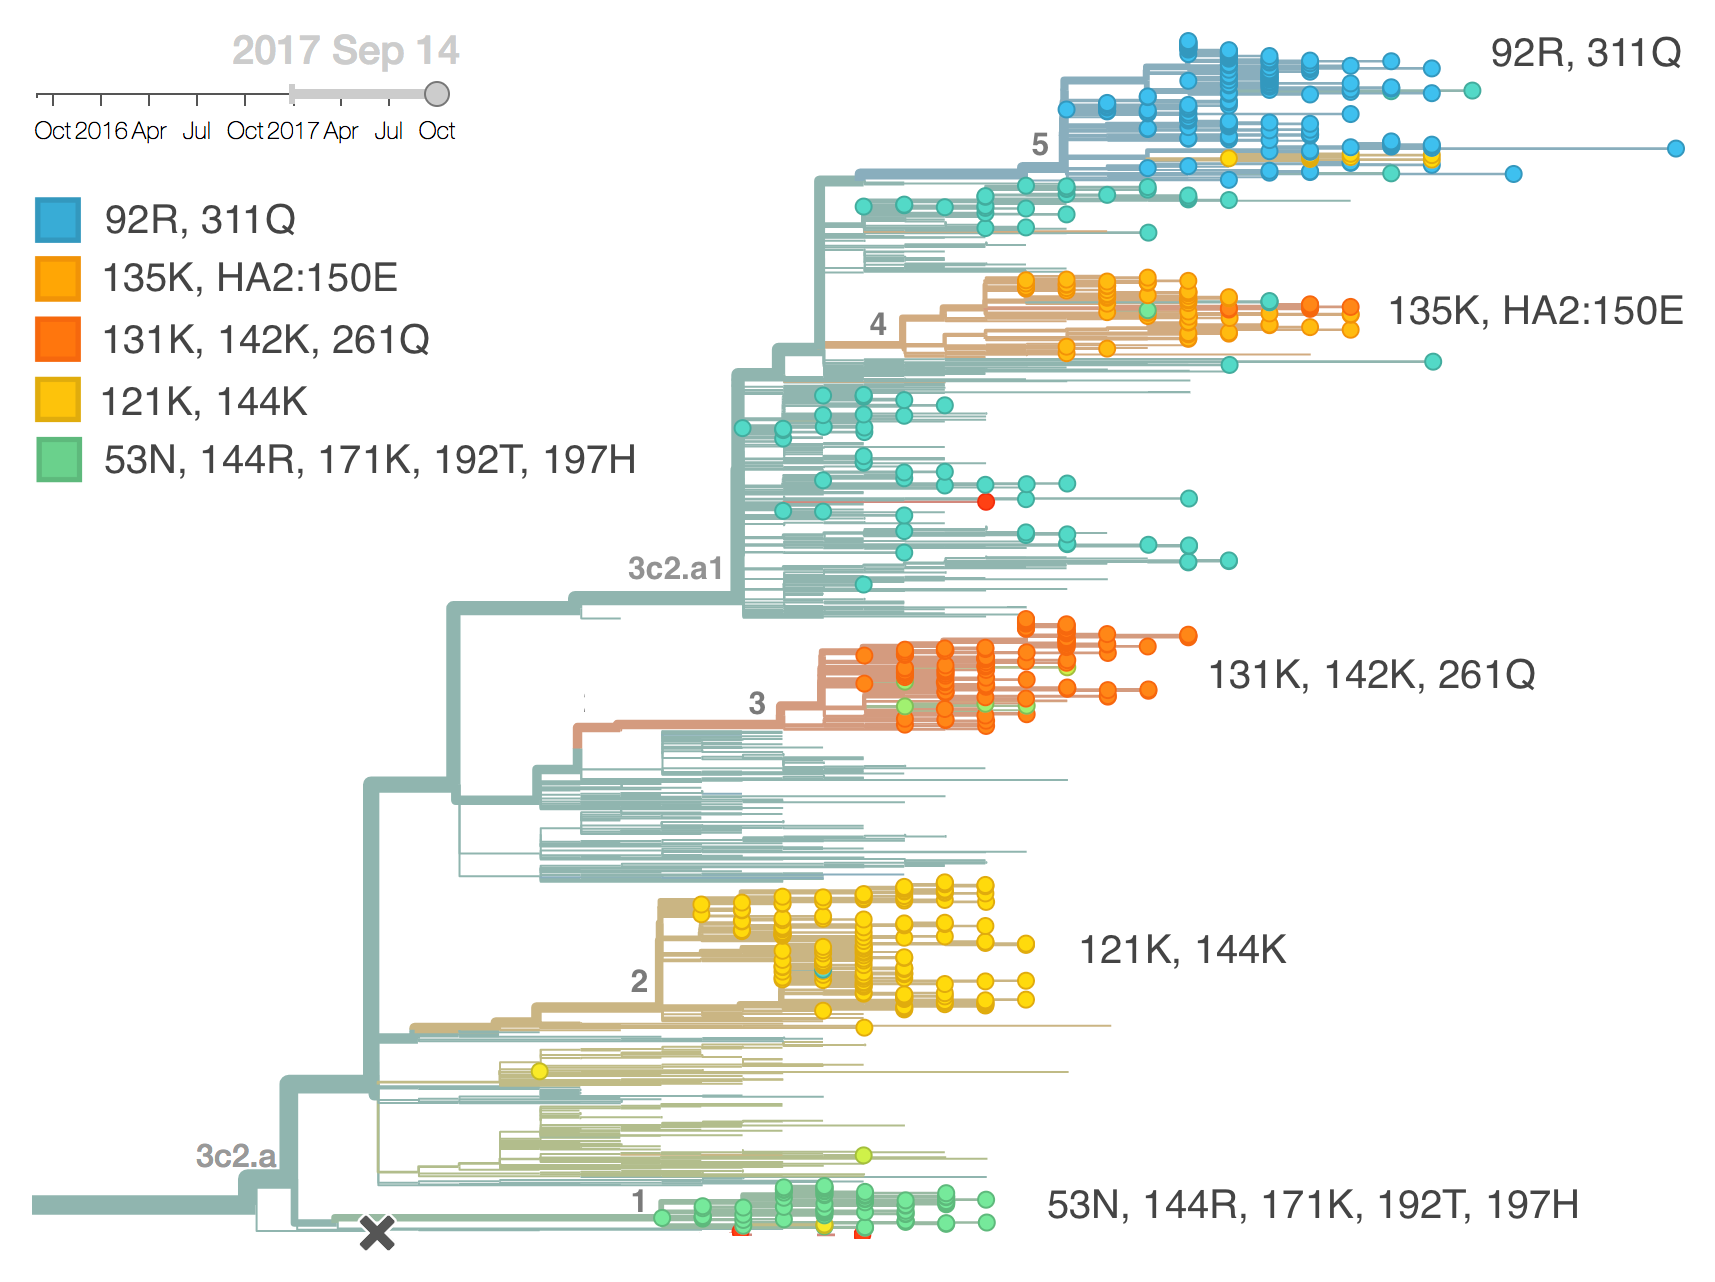
\includegraphics[width=0.8\textwidth]{../figures/sep-2017/h3n2_tree.png}
  \caption{\textbf{H3N2 / 3c2.a phylogeny colored by genotype.} Colors are chosen to highlight the clades 1--5. Clades are in reverse order, that is clade 5 is on top, clade 1 is at the bottom.
  }
  \label{H3N2_tree}
\end{figure}


We observe substantial diversification within the 3c2.a clade over the
past year. There are 5 major subclades within 3c2.a that have reached
appreciable frequency. These clades are characterized by the following
mutations and highlighed in the phylogenetic tree in \FIG{H3N2_tree}:

\begin{enumerate}
\item  Clade 1: 53N, 144R, 171K, 192T, 197H
\item  Clade 2: 121K, 144K
\item  Clade 3: 131K, 142K, 261Q
\item  Clade 4: 135K, HA2:150E
\item  Clade 5: 92R, 311Q
\end{enumerate}

All of these clades possess mutations at previously characterized
epitope sites. We will refer to these clades as clade 1--5.

All of these clades have risen in frequency and are now competing with
one another, see \FIG{H3N2_mutations}. Clade 1 (53N, 144R, 171K, 192T, 197H) is highly derived in
terms of sequence, but is at low frequency globally (currently less than
1\%) despite making up the a substantial fraction of 2017 Oceania
viruses. Clade 2 (121K, 144K) is beginning to decline in frequency and
is now at \textasciitilde{}21\% global frequency. Clade 3 (131K, 142K,
261Q) and clade 4 (135K, HA2:150E) have each slowly climbed to
approximately 20\% frequency. However, clade 5 (92R, 311Q) has recently
increased to 39\% in global frequency.

\begin{figure}[h!]
  \centering
  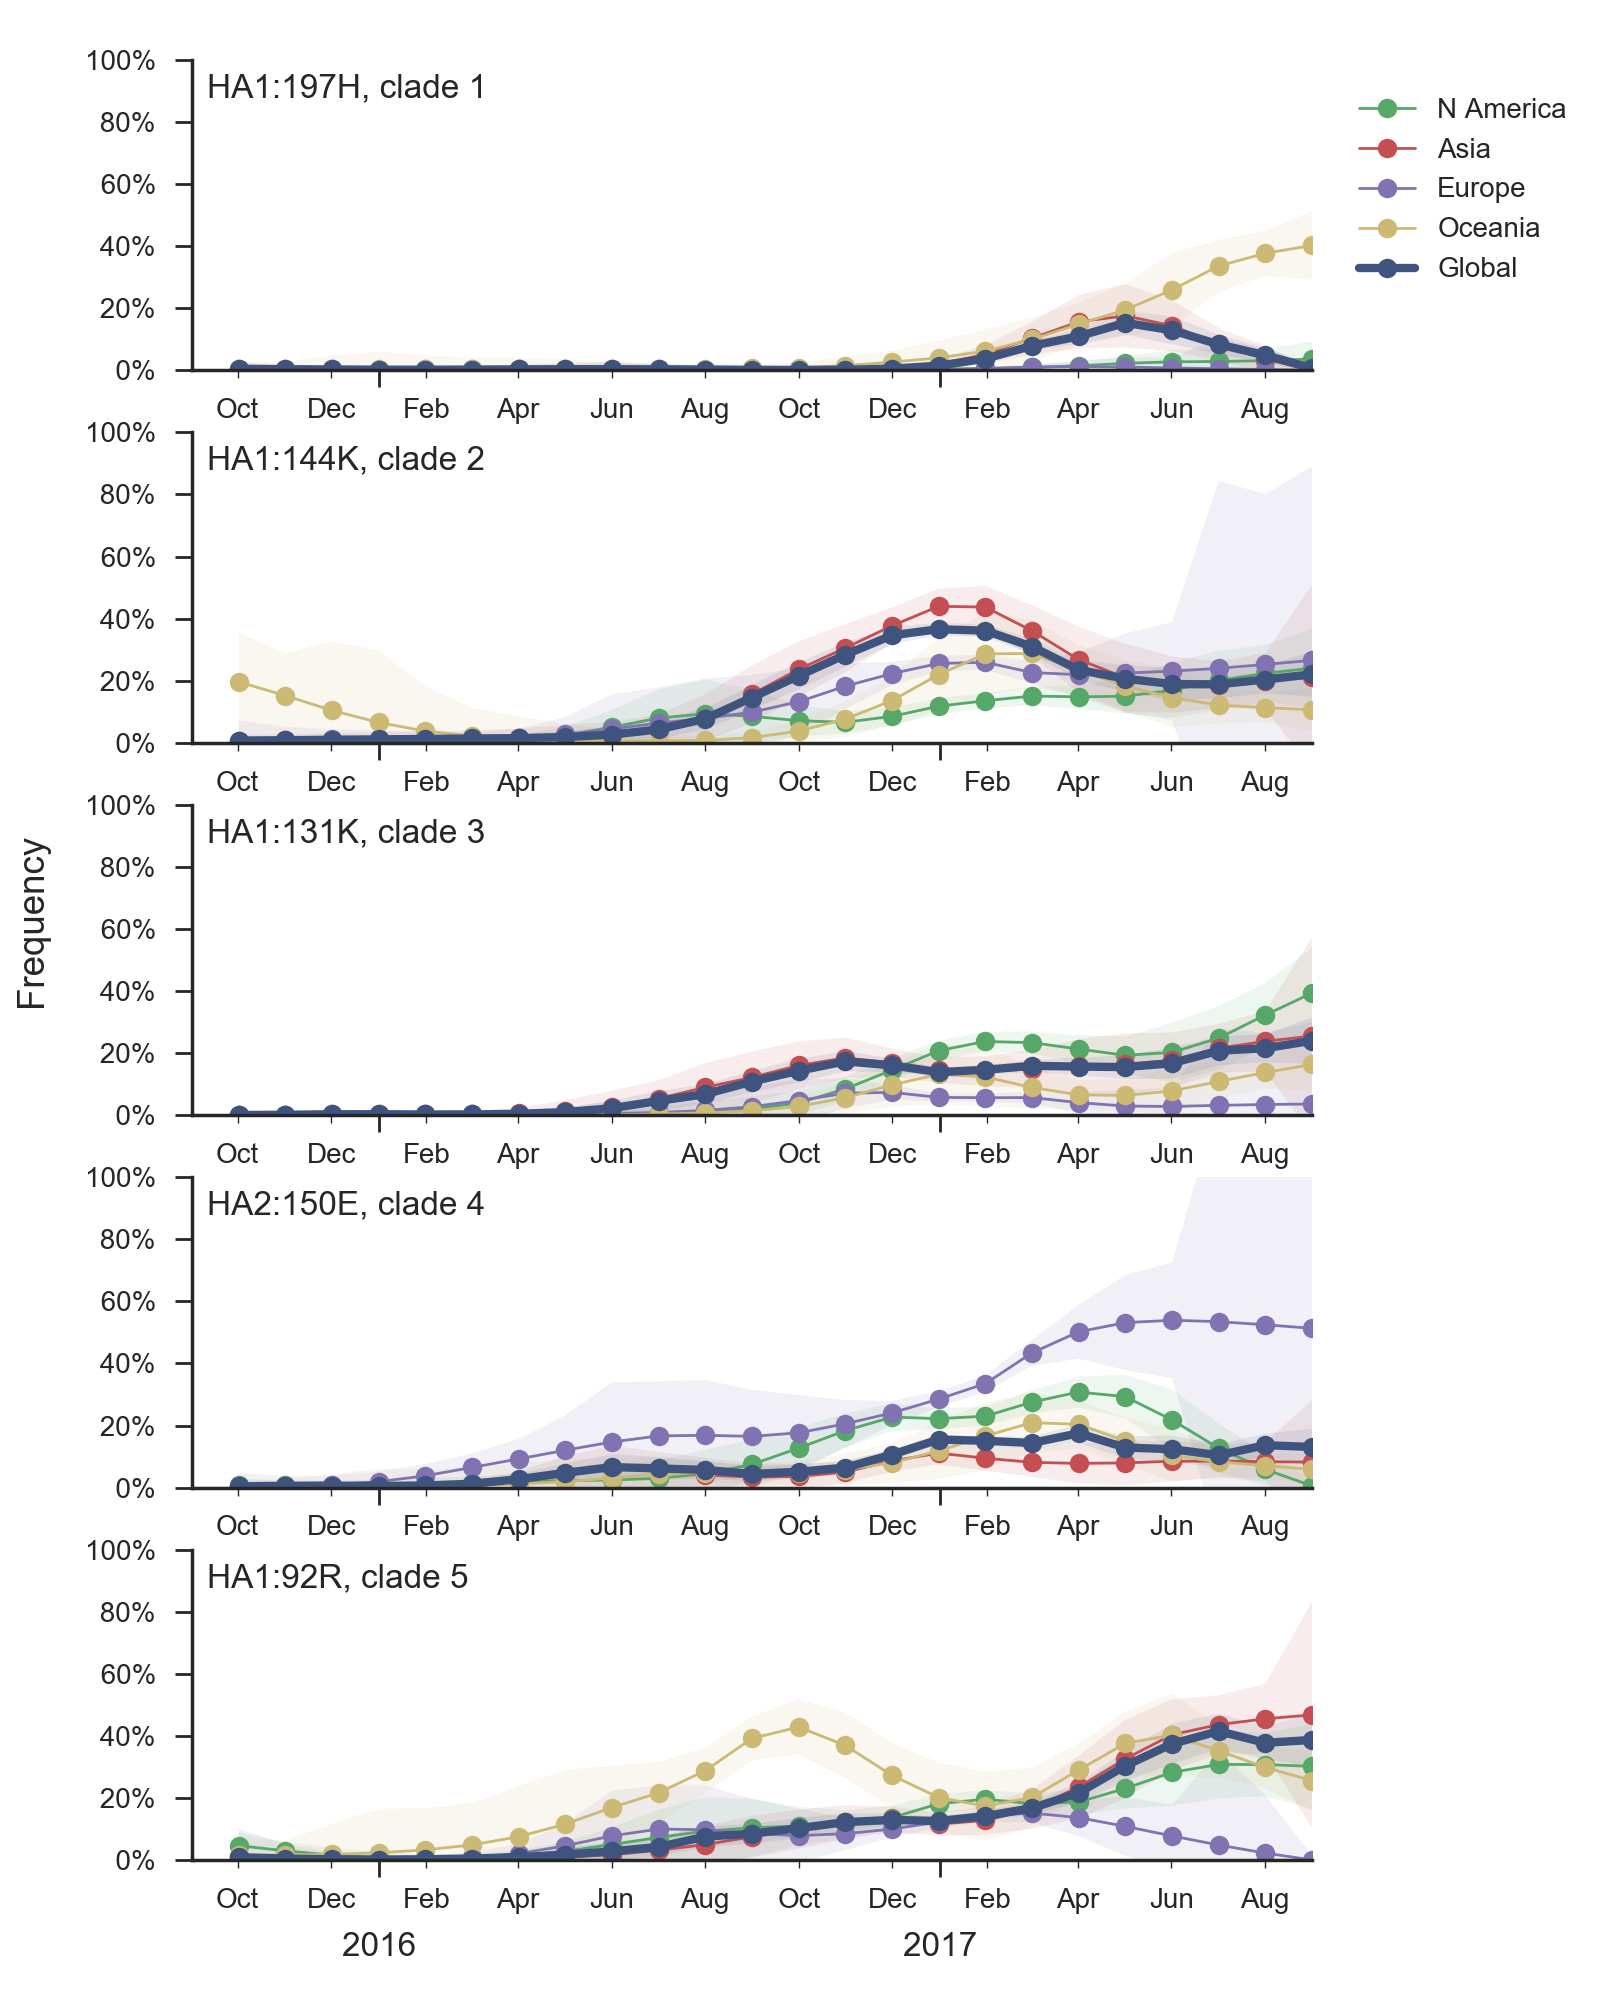
\includegraphics[width=0.95\textwidth]{../figures/sep-2017/h3n2_mutations.png}
  \caption{\textbf{Frequency trajectories of 3c2.a subclades.}
  We estimate frequencies of different clades based on sample counts and collection dates.
  We use a Brownian motion process prior to smooth frequencies from month-to-month.
  Transparent bands show an estimate the 95\% confidence interval based on sample counts.
  }
  \label{H3N2_mutations}
\end{figure}



\clearpage
\begin{figure}[h!]
  \centering
  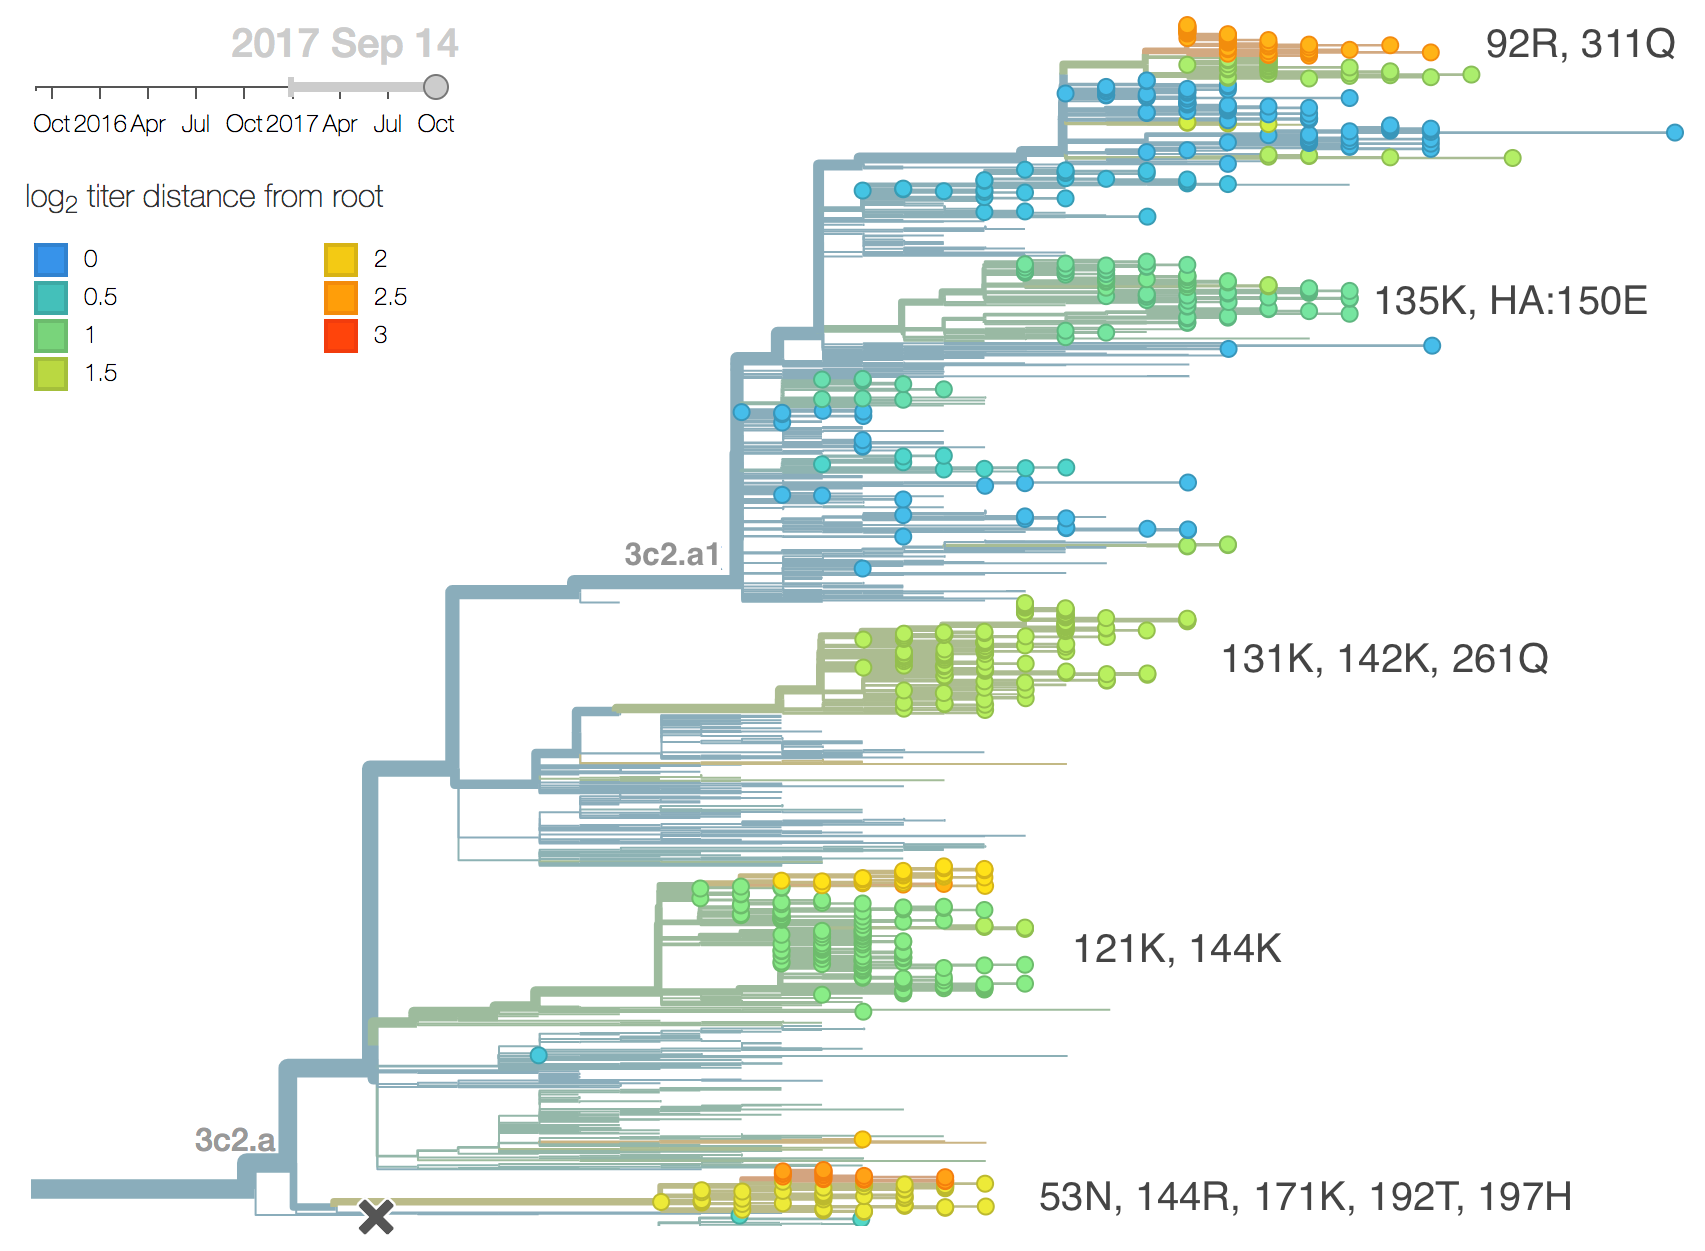
\includegraphics[width=1.0\textwidth]{../figures/sep-2017/h3n2_tree_titer_model.png}
  \caption{\textbf{H3N2 phylogeny colored by antigenic advance.}
  Each panel shows model estimates of antigenic divergence relative to the root of the tree, which is similar to the titer drop relative to A/HongKong/5738/2014.
  Cooler color indicates greater antigenic similarity (less titer drop going from homologous to heterologous titers).
  }
  \label{H3N2_tree_titer_model}
\end{figure}


All 5 of these clades appear somewhat drifted according to antigenic
analysis Neher et al \cite{neher2015prediction} of HI measurements provided by the Influenza Division at the US CDC, see \FIG{H3N2_tree_titer_model}.
With antigenic differences estimated between 0.5 units and 2.0 units.


The mutation T135K has appeared independently in clades 2, 4 and 5 and is now globally at 40\% frequency.
The most rapidly growing clade carries mutations
N121K/K92R/H311Q/E62G/R142G/T135K. This is a subclade of clade 5 above
with addition of 62G, 142G and 135K. The model fit to the antigenic data
estimates that this subclade of clade 5 has drifted by 2.2 antigenic
units, 1 of which is associated with the E62G/R142G mutations and 1.2
with the T135K mutation (on this background), see \FIG{H3N2_135K}.
Note, however, that there
is no evidence of antigenic evolution in the FRA data (one data point
only). A small sister clade with mutation T135N (also part of clade 5)
recently developed. Taken together, changes at position 135 likely have
selective origin.

\begin{figure}[h!]
  \centering
  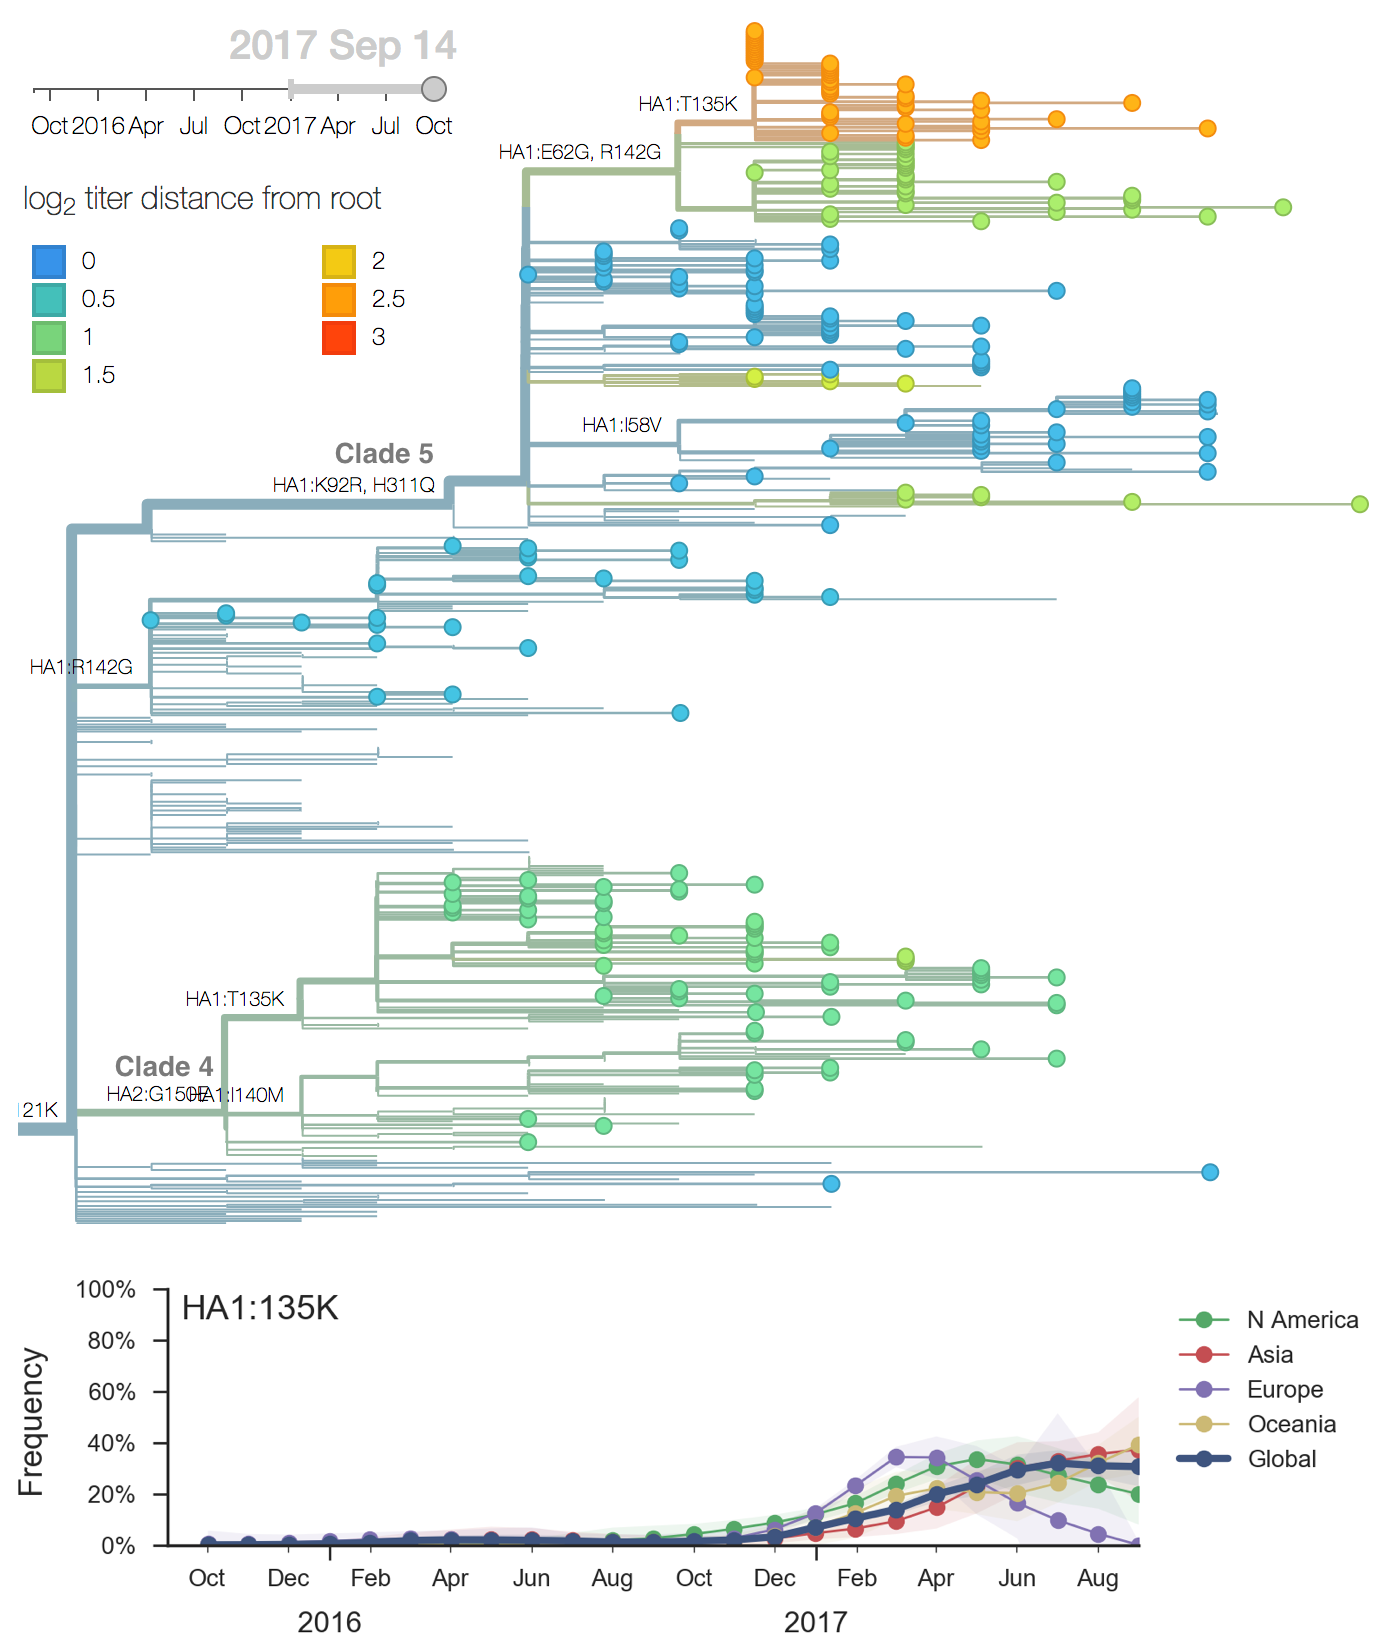
\includegraphics[width=0.8\textwidth]{../figures/sep-2017/h3n2_tree_135k.png}
  \caption{\textbf{Zoom into clade 5, colored by antigenic advance.} A subclade with a T135K mutation has recently risen in frequency and has drifted $>$2 antigenic units.
  }
  \label{H3N2_135K}
\end{figure}

Clades 1,2, and 3 are part of 3c2.a but outside of the 3c2.a1 subclade.
Clade 3 with T131K/R142K mutations continues to be common in China (but
not in South Asia) with an embedded cluster of South and North American
isolates from last summer. Subclusters within this clade have been
expanding recently, but there is little evidence for antigenic evolution
in the HI or FRA data. The 131K substitution is not seen outside this
clade.

Clade 1 with substitutions N31S/D53N/S144R/N171K/I192T/Q197H was
observed globally over the past 9 month but is now decreasing everywhere
except Oceania HI data and the model fit suggest a moderate (4-fold,
about 2 antigenic units) titer drop relative to A/HongKong/4801/2014.
Despite the titer drop, this calde seems to be outcompeted almost
everywhere.

The most notable subclade of 3c3.a is a clade carrying the mutation
F193S. However, this clade along with its sister clades has been
decreasing in recent month and it doesn't show a consistent signal of
antigenic change. The F193D mutations is observed sporadically within
the 3c2.a clade as well.

% \begin{figure}[h!]
%   \centering
%   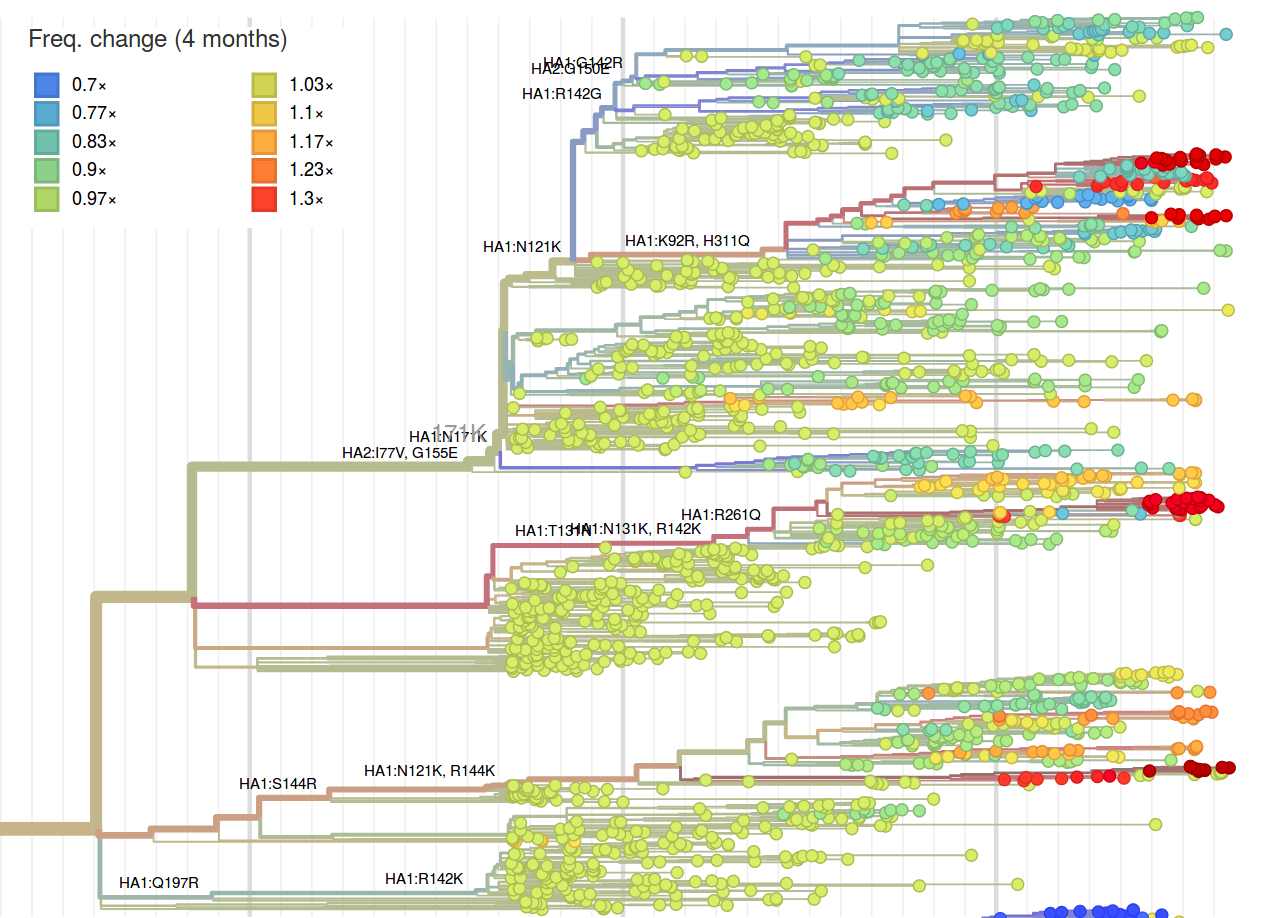
\includegraphics[width=1.0\textwidth]{../figures/sep-2017/h3n2_3c2a.png}
%   \caption{\textbf{Recent frequency changes.} The tree, zoomed into clade 3c2.a, is colored by change in clade frequency over the past 4 month.
%   }
%   \label{H3N2_135K}
% \end{figure}

In summary, we think that the clade most likely to increase further in
frequency is the E62G/R142G/T135K clade. However, two other clades
(T131K/R142K and 144K) have similar potential. The former has very
rapidly growing subclade, the latter rose rapidly last year and has a
slightly higher LBI than the other two.


\clearpage
\section*{A/H1N1pdm}
\addcontentsline{toc}{section}{A/H1N1pdm}

\textbf{A clade comprising mutations S74R and I295V has recently risen
to \textgreater{}90\% global frequency. Although it shows no antigenic
distinction by ferret HI data, the rapidity of its rise suggests a
selective origin.}

We base our primary analysis on a set of viruses collected between Oct
2015 and Aug 2017, comprising approximately 100 viruses per month during
relevant months of 2017, see \FIG{H1N1pdm_counts}. We use all available data when estimating
frequencies of mutations and weight samples appropriately by regional
population size and relative sampling intensity to arrive at a
putatively unbiased global frequency estimate. Phylogenetic analyses are
based on a representative sample of about 2000 viruses.

\begin{figure}[H]
  \centering
  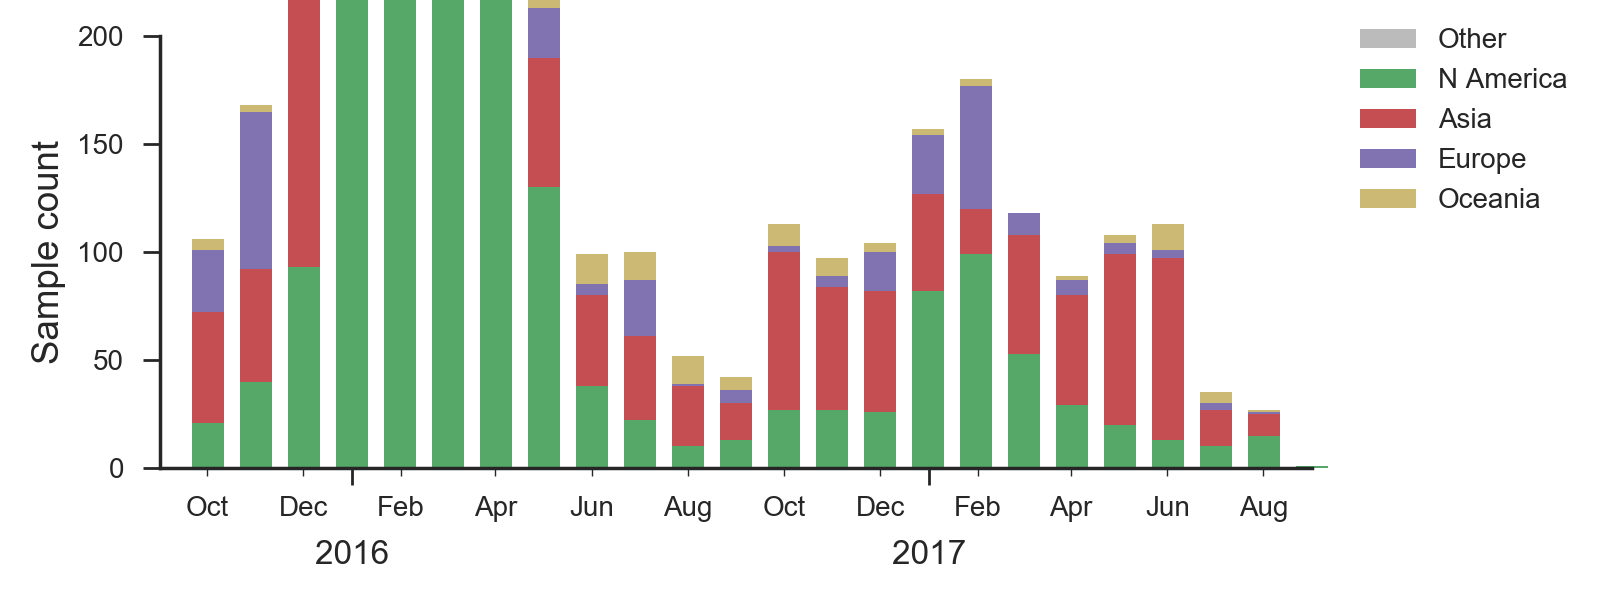
\includegraphics[width=0.95\textwidth]{../figures/sep-2017/h1n1pdm_counts.png}
  \caption{\textbf{A/H1N1pdm sample counts through time and across regions.}}
  \label{H1N1pdm_counts}
\end{figure}

H1N1pdm recently underwent a selective sweep of the 6b.1 clade
comprising mutations S162N and I216T. Nearly all currently circulating
H1N1pdm viruses are clade 6b.1. The H1N1pdm vaccine strain was updated
in Sep 2016 to match 6b.1 viruses.

There has been little diversification within clade 6b.1 with a couple
notable exceptions. There is a clade comprising mutations S74R and I295V
that has been very successful. Within this clade, there is a more recent
subclade with the additional mutation S164T.

\begin{figure}[H]
  \centering
  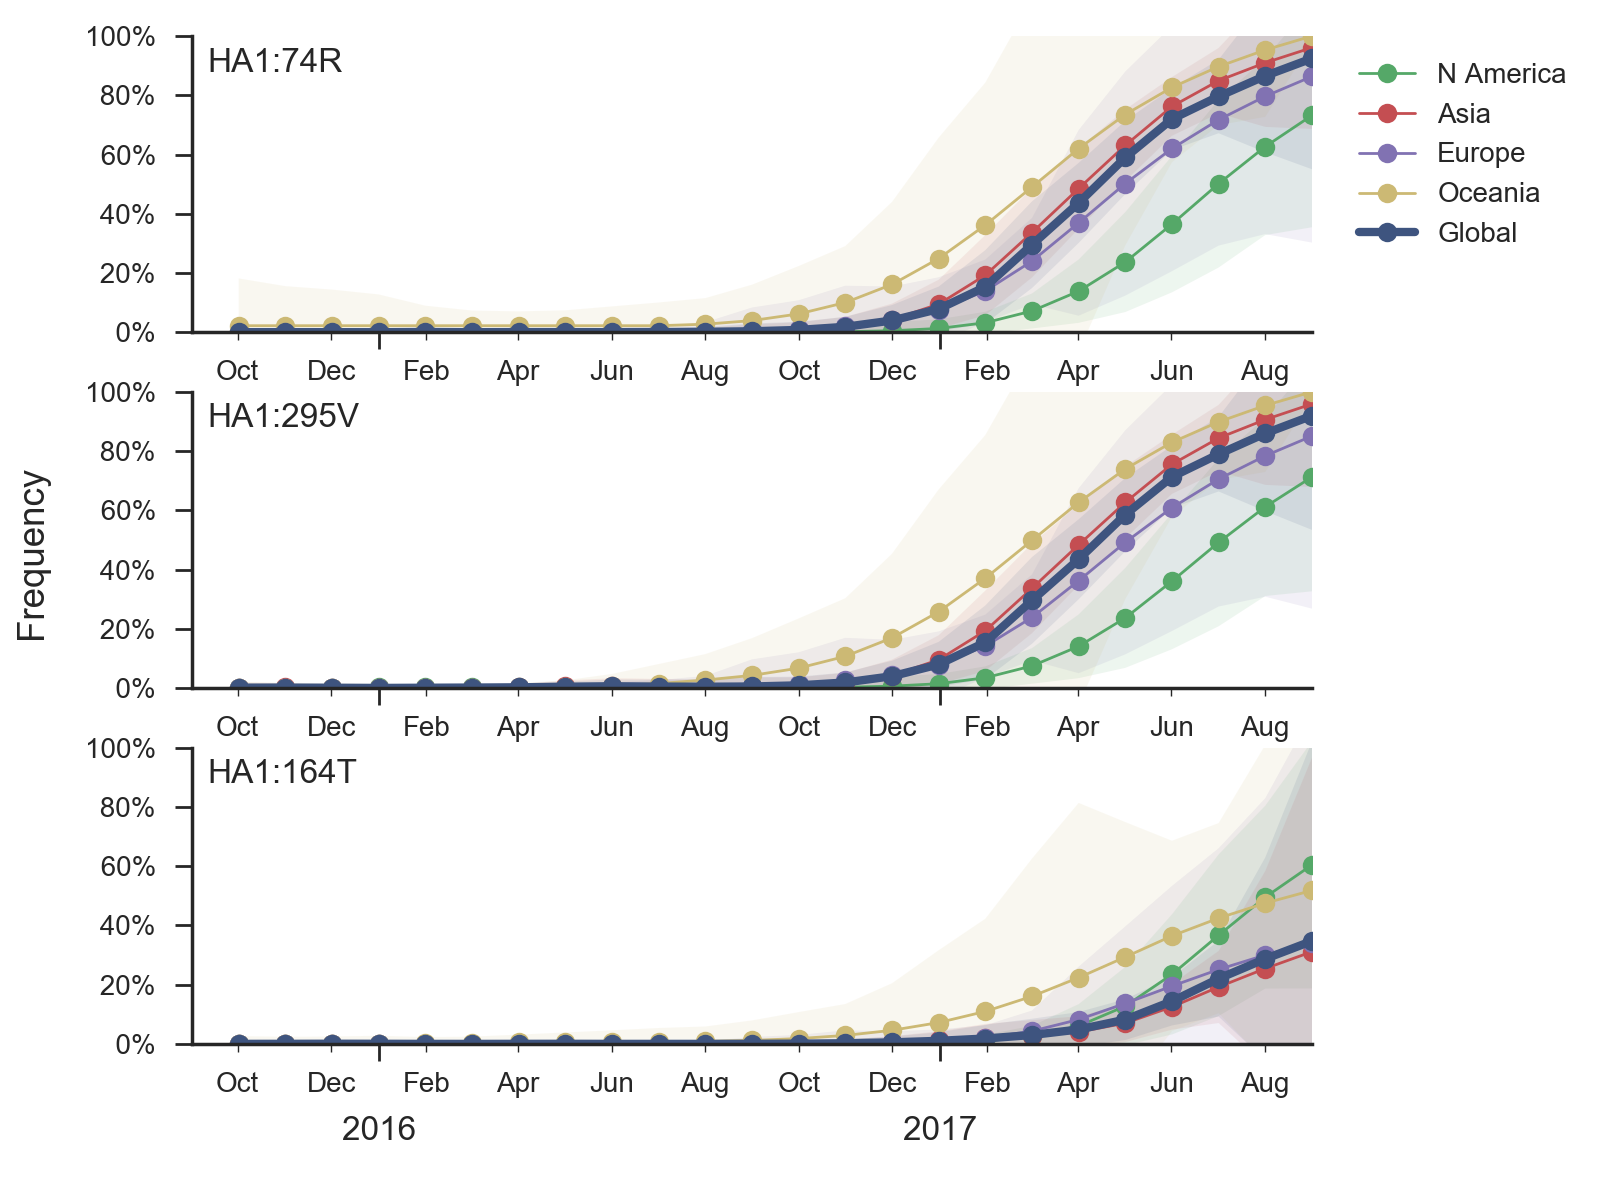
\includegraphics[width=0.95\textwidth]{../figures/sep-2017/h1n1pdm_mutations.png}
  \caption{\textbf{Frequency trajectories of recent mutations in A/H1N1pdm viruses.}  }
  \label{H1N1pdm_clades}
\end{figure}

The S74R and I295V clade has risen rapidly in frequency starting around
Jan 2017. This clade has been very successful and is now at
approximately 92\% global frequency. Within this clade the subclade
comprising S164T has risen in frequency from April 2017 and is now at
approximately 35\% global frequency, see \FIG{H1N1pdm_clades}

Other mutations have appeared within 6b.1 viruses including S183P, R205K
and I324V, but none of these have been very successful and are now
declining in response to the rise of S74R and I295V.

\clearpage
\begin{figure}[H]
  \centering
  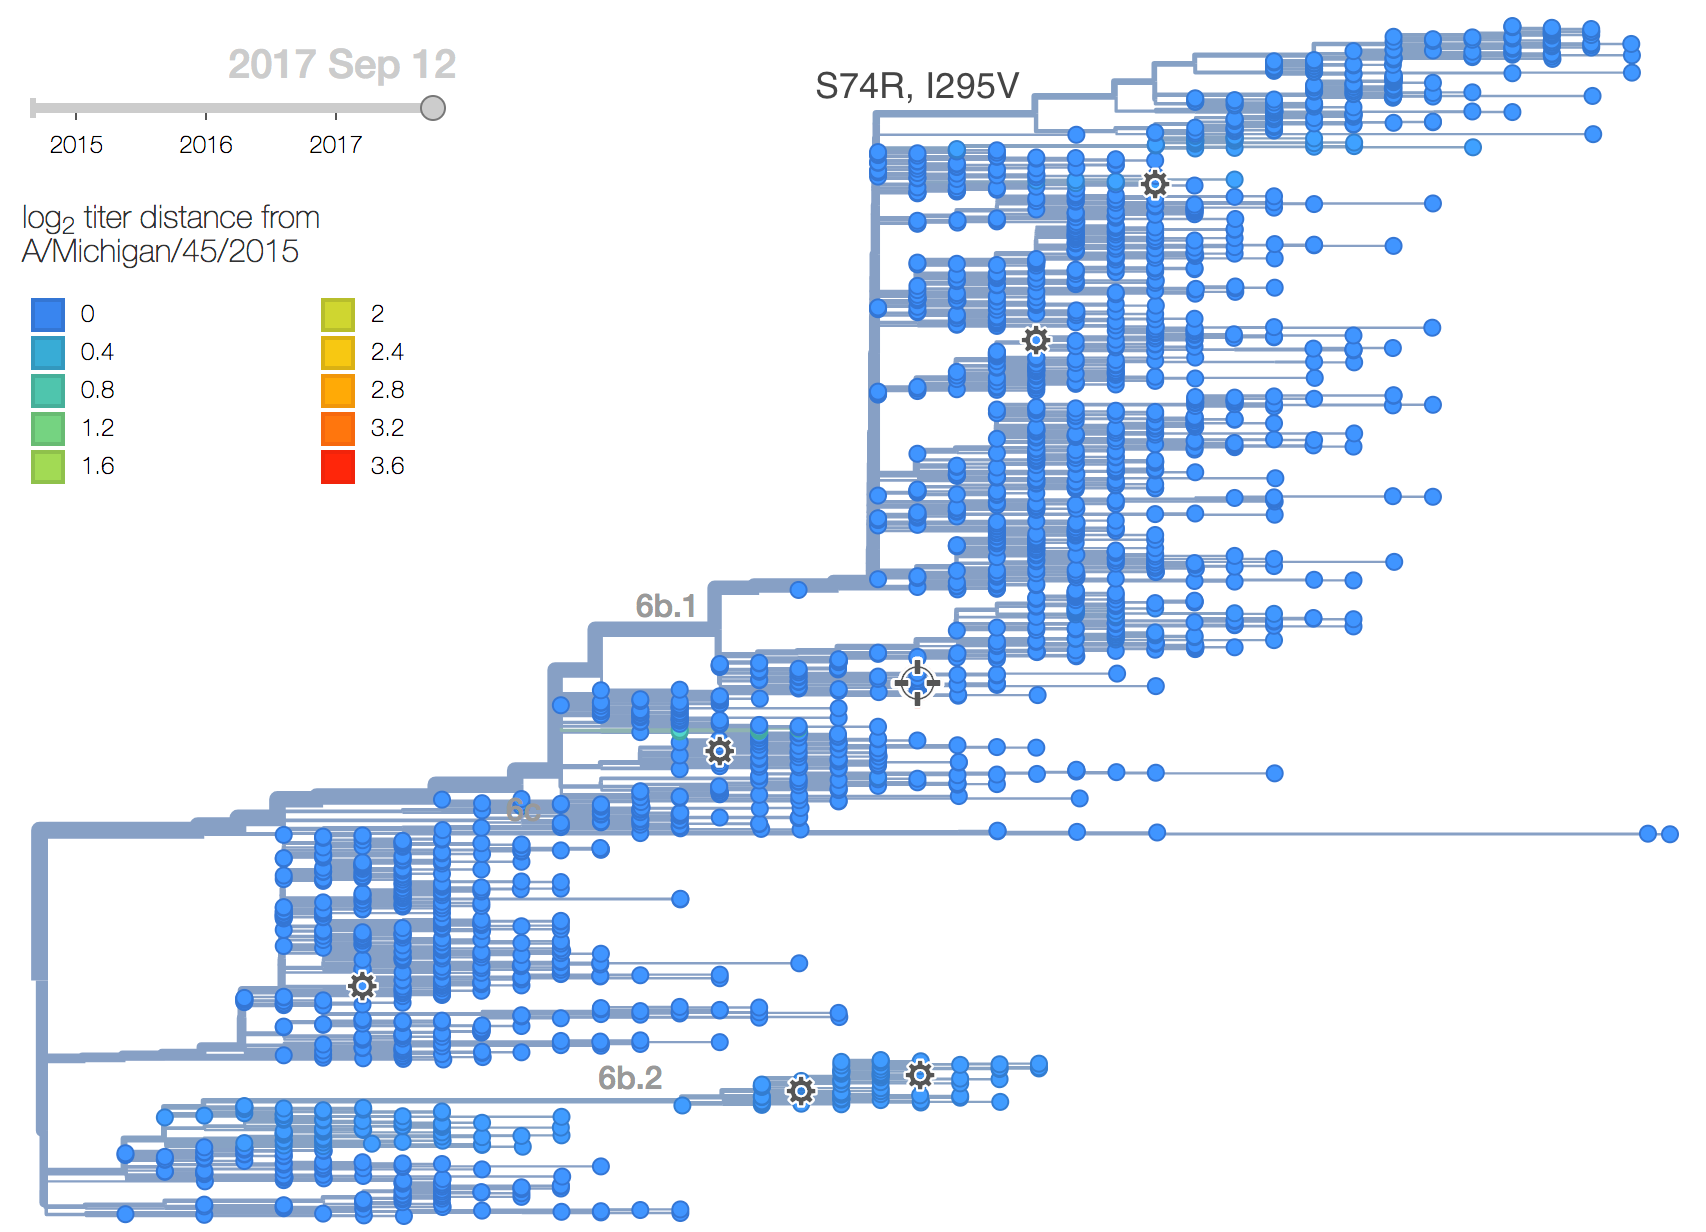
\includegraphics[width=0.9\textwidth]{../figures/sep-2017/h1n1pdm_tree_titer_model.png}
  \caption{\textbf{Antigenic distance from A/Michigan/45/2015.} No antigenic variation is picked up by the model.
  }
  \label{H1N1pdm_mutations}
\end{figure}
Antigenic analysis using HI measurements provided by the Influenza
Division at the US CDC fails to show any distinction within recently
circulating H1N1pdm viruses. Like the clades 6b and 6b.1 clade before
it, the new S74R and I295V clade does not show any titer drop despite
there being ample measurements.


\begin{figure}[H]
  \centering
  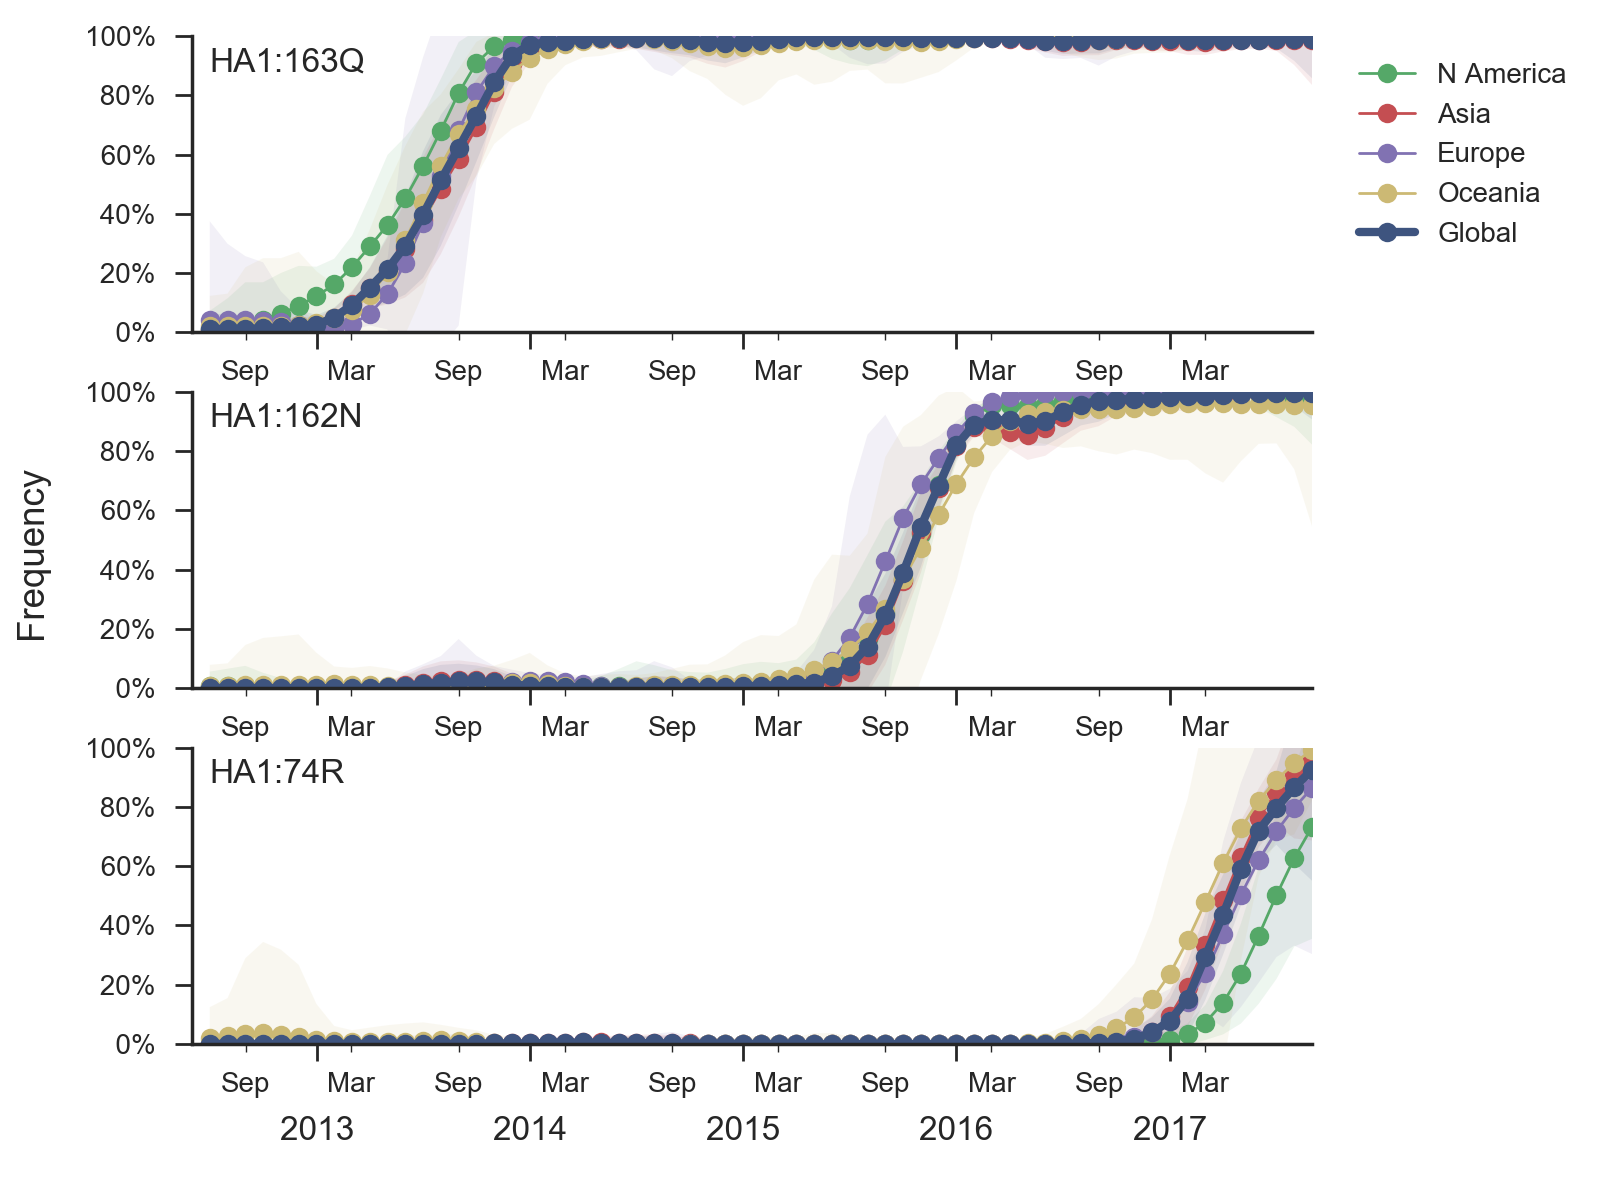
\includegraphics[width=0.9\textwidth]{../figures/sep-2017/h1n1pdm_mutations_6b_6b1.png}
  \caption{\textbf{Sequential rapid replacement of clades in A/H1N1pdm.} The latest rapid rise of 74R took place at similar or greater speed as the spread of 162N.
  }
  \label{H1N1pdm_mutations}
\end{figure}
It was previously observed that clade 6b viruses with mutation K163Q
showed decreased titers in a subset of adult human sera due to
immunodominance effects, despite continued high titers in ferret sera
(\href{http://www.pnas.org/content/111/44/15798}{Linderman et al 2014}).
Importantly, the new S74R and I295V clade has spread at a similarly
rapid rate as did clades 6b and 6b.1. This rate of spread and
displacement of existing viral diversity is consistent with a selective
origin.



\emph{Given current patterns of growth and decline it is almost certain
that the S74R and I295V clade will dominant in a years time. Although
there is no antigenic effect visible via HI from ferret antisera, the
rapidity of the rise of S74R and I295V suggests a selective origin. We
would suggest a detailed examination of human serological data as it's
already been established that human serology may differ from ferret
serology in H1N1pdm viruses.}

\clearpage
%%% B/Victoria %%%
\section*{B/Vic}
\addcontentsline{toc}{section}{B/Vic}

\textbf{A clade with a two amino acid deletion 162-/163- has altered
serological properties and is increasing in frequency, albeit slowly.
Two other clades (carrying mutations K209N and V87A/I175V) have
increased in frequency moderately.}

We base our primary analysis on a set of viruses collected between Oct
2015 and Aug 2017, comprising between 50 and 250 viruses per month
during relevant months of 2017, see \FIG{Vic_counts}. We use all available data when
estimating frequencies of mutations and weight samples appropriately by
regional population size and relative sampling intensity to arrive at a
putatively unbiased global frequency estimate. Phylogenetic analyses are
based on a representative sample of about 2000 viruses.

\begin{figure}[H]
  \centering
  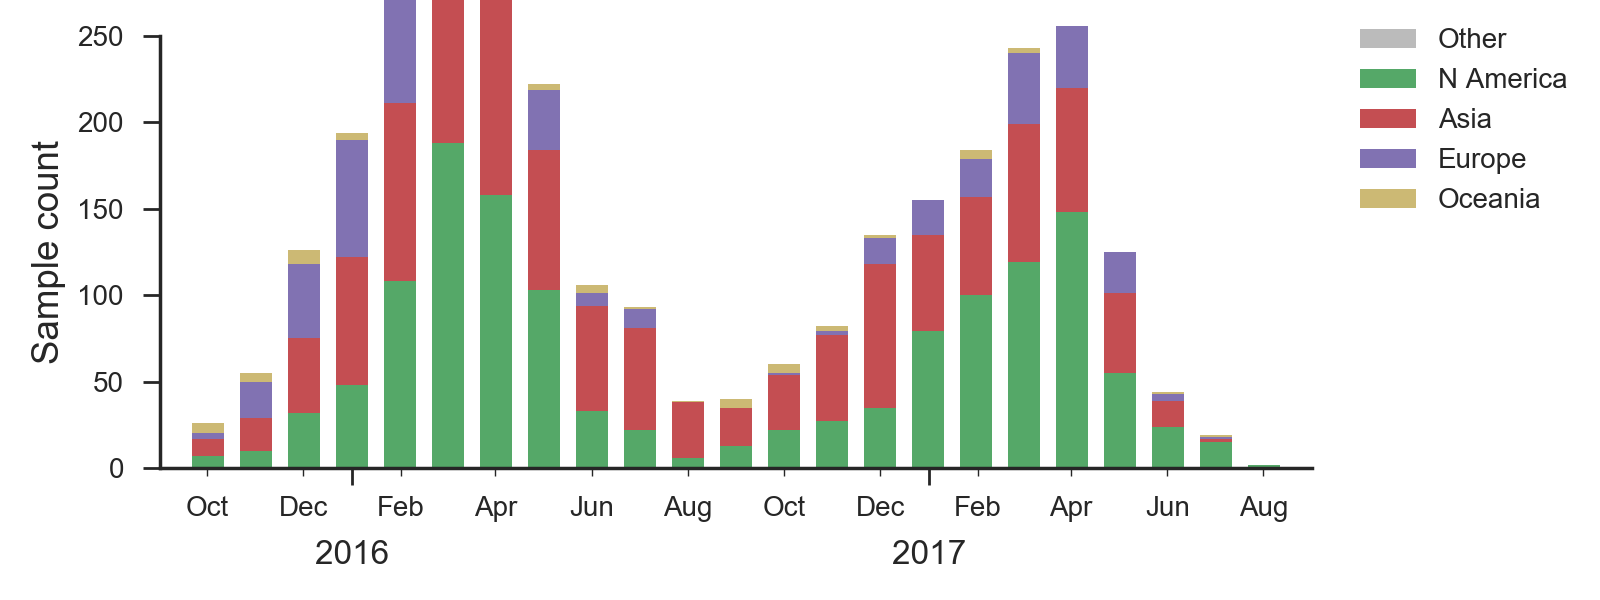
\includegraphics[width=0.95\textwidth]{../figures/sep-2017/vic_counts.png}
  \caption{\textbf{Sample counts through time and across regions.}
  This is a stacked bar plot, so that in good months there are $\sim$200 total samples.
  }
  \label{Vic_counts}
\end{figure}
\clearpage
\begin{figure}[H]
  \centering
  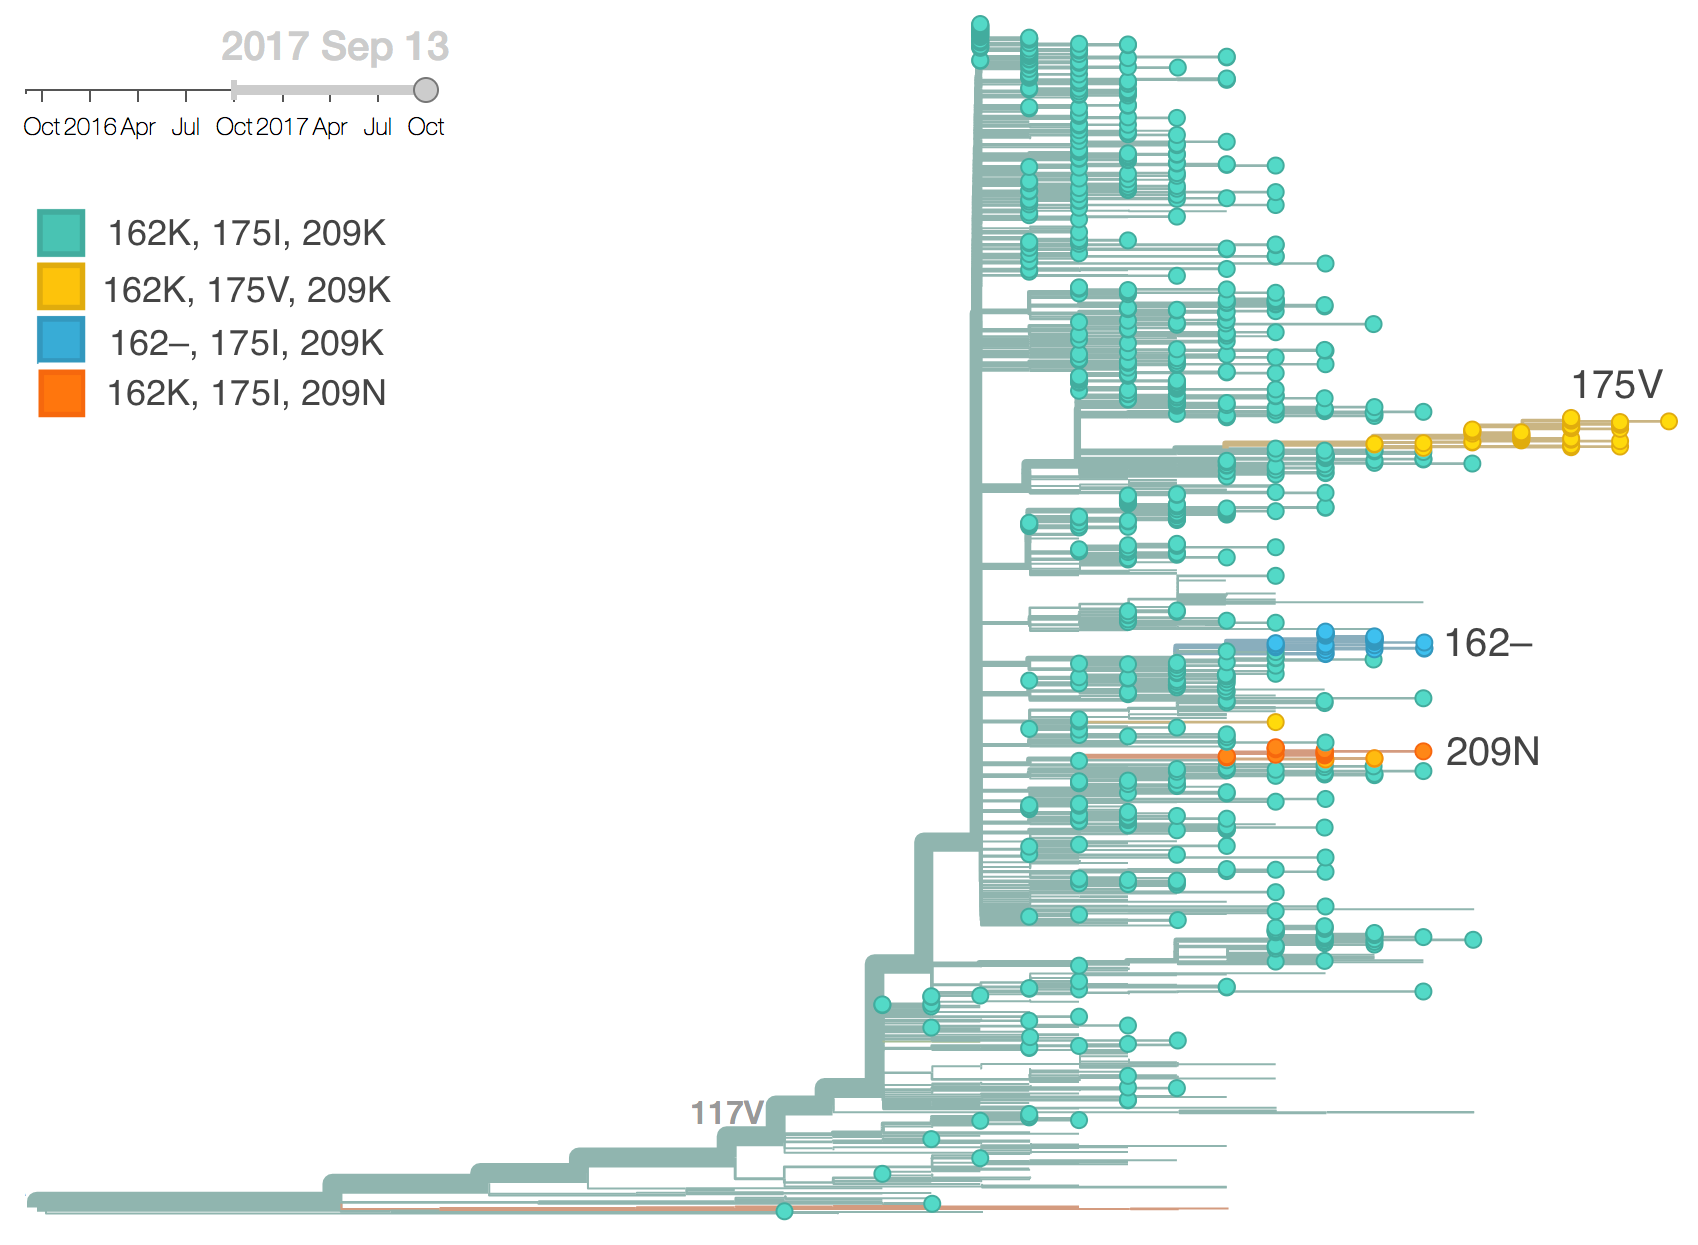
\includegraphics[width=0.95\textwidth]{../figures/sep-2017/vic_tree.png}
  \caption{\textbf{B/VIC -- Phylogenetic tree colored by genotype as positions 162, 175, 209.}
  }
  \label{Vic_tree}
\end{figure}
The mutation I117V has continued its slow ascent in frequency as is now
\textgreater{}99\% in the global population. Within this clade there is
relatively little circulating genetic diversity. The only clades of note
are a small clade with mutations I180V, D129G and deletions K162- and
K163-, another small clade with mutations V87A and I175V and a third
small clade with mutation K209N.

\clearpage
\begin{figure}[H]
  \centering
  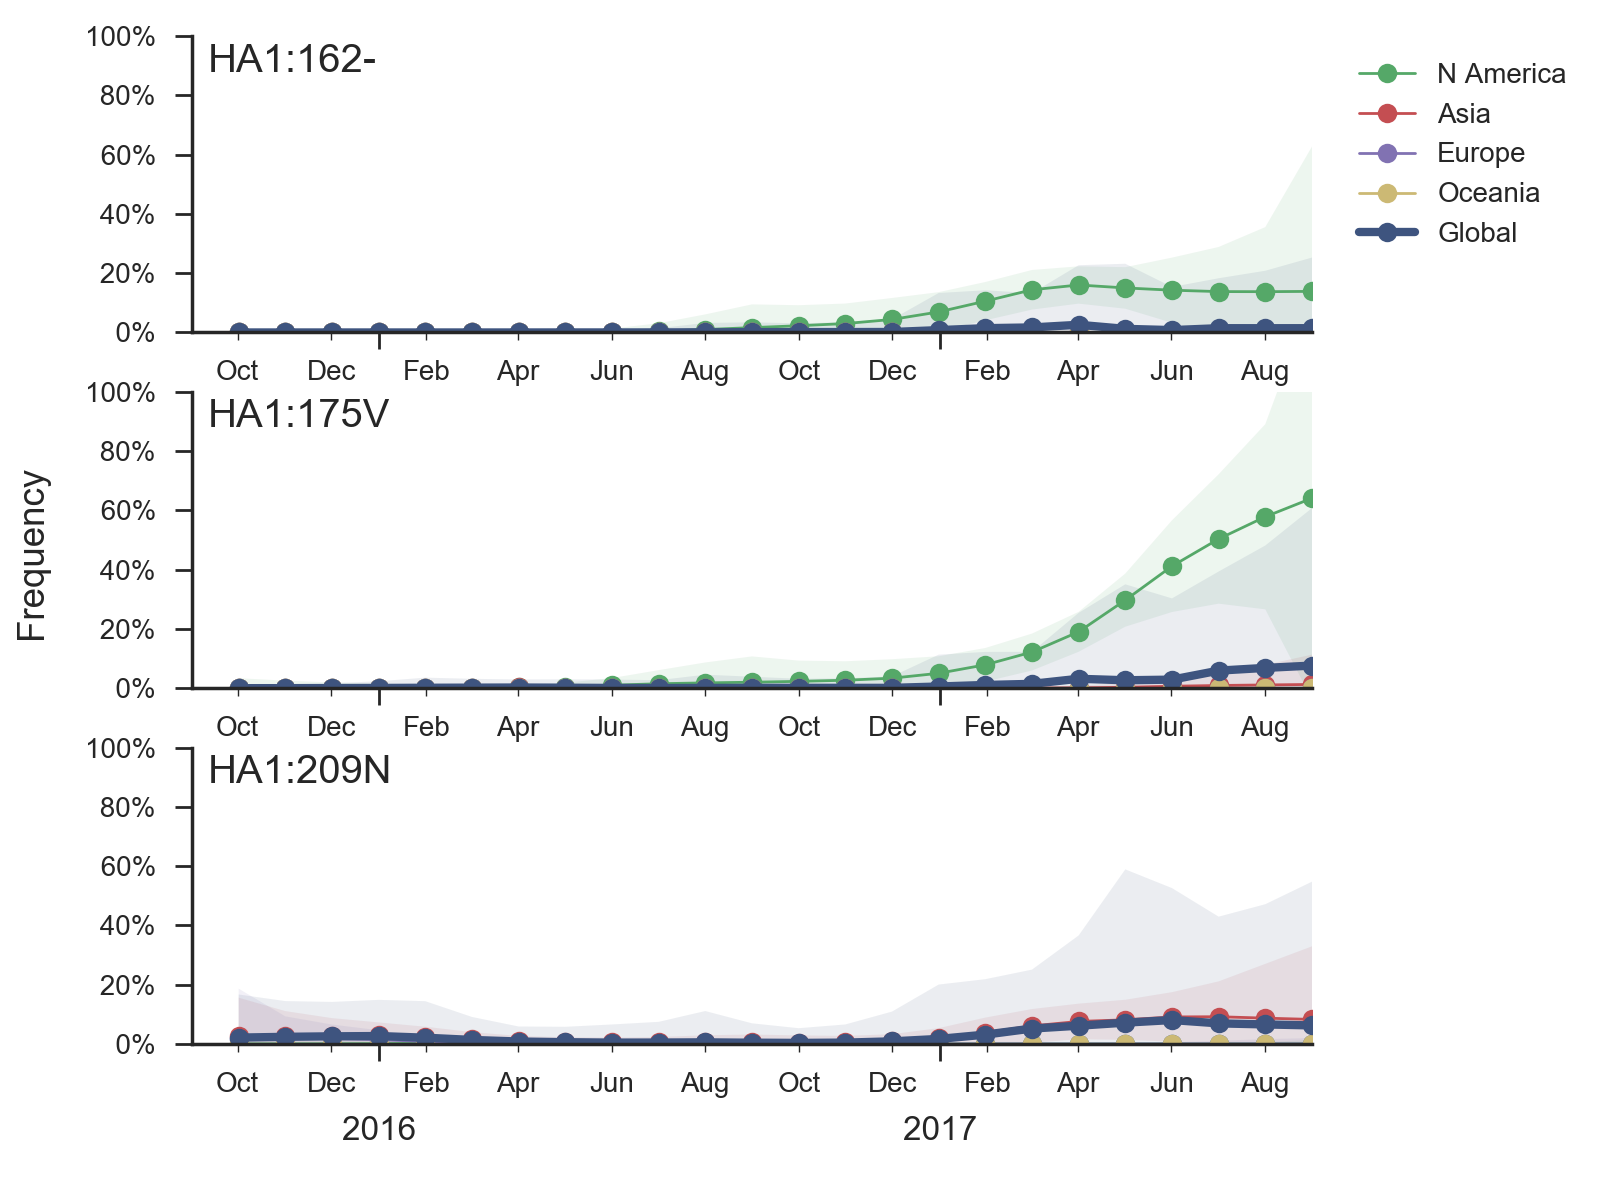
\includegraphics[width=0.95\textwidth]{../figures/sep-2017/vic_mutations.png}
  \caption{\textbf{Frequency trajectories of B/Vic variants.}
  We estimate frequencies of different clades based on sample counts and collection dates.
  We use a Brownian motion process prior to smooth frequencies from month-to-month.
  Transparent bands show an estimate the 95\% confidence interval based on sample counts.
  }
  \label{Vic_mutations}
\end{figure}
The clade bearing 129G, 162--, 163-- and 180V has remained at low
frequency globally with current global estimates at
\textasciitilde{}4\%, see \FIG{Vic_mutations}. The clade bearing 87A and 175V has increased in
frequency substantially in North America but remains low in the rest of
the world. The clade bearing 209N has been more successful, approaching
15\% globally and circulating in Asia.

\clearpage
\begin{figure}[H]
  \centering
  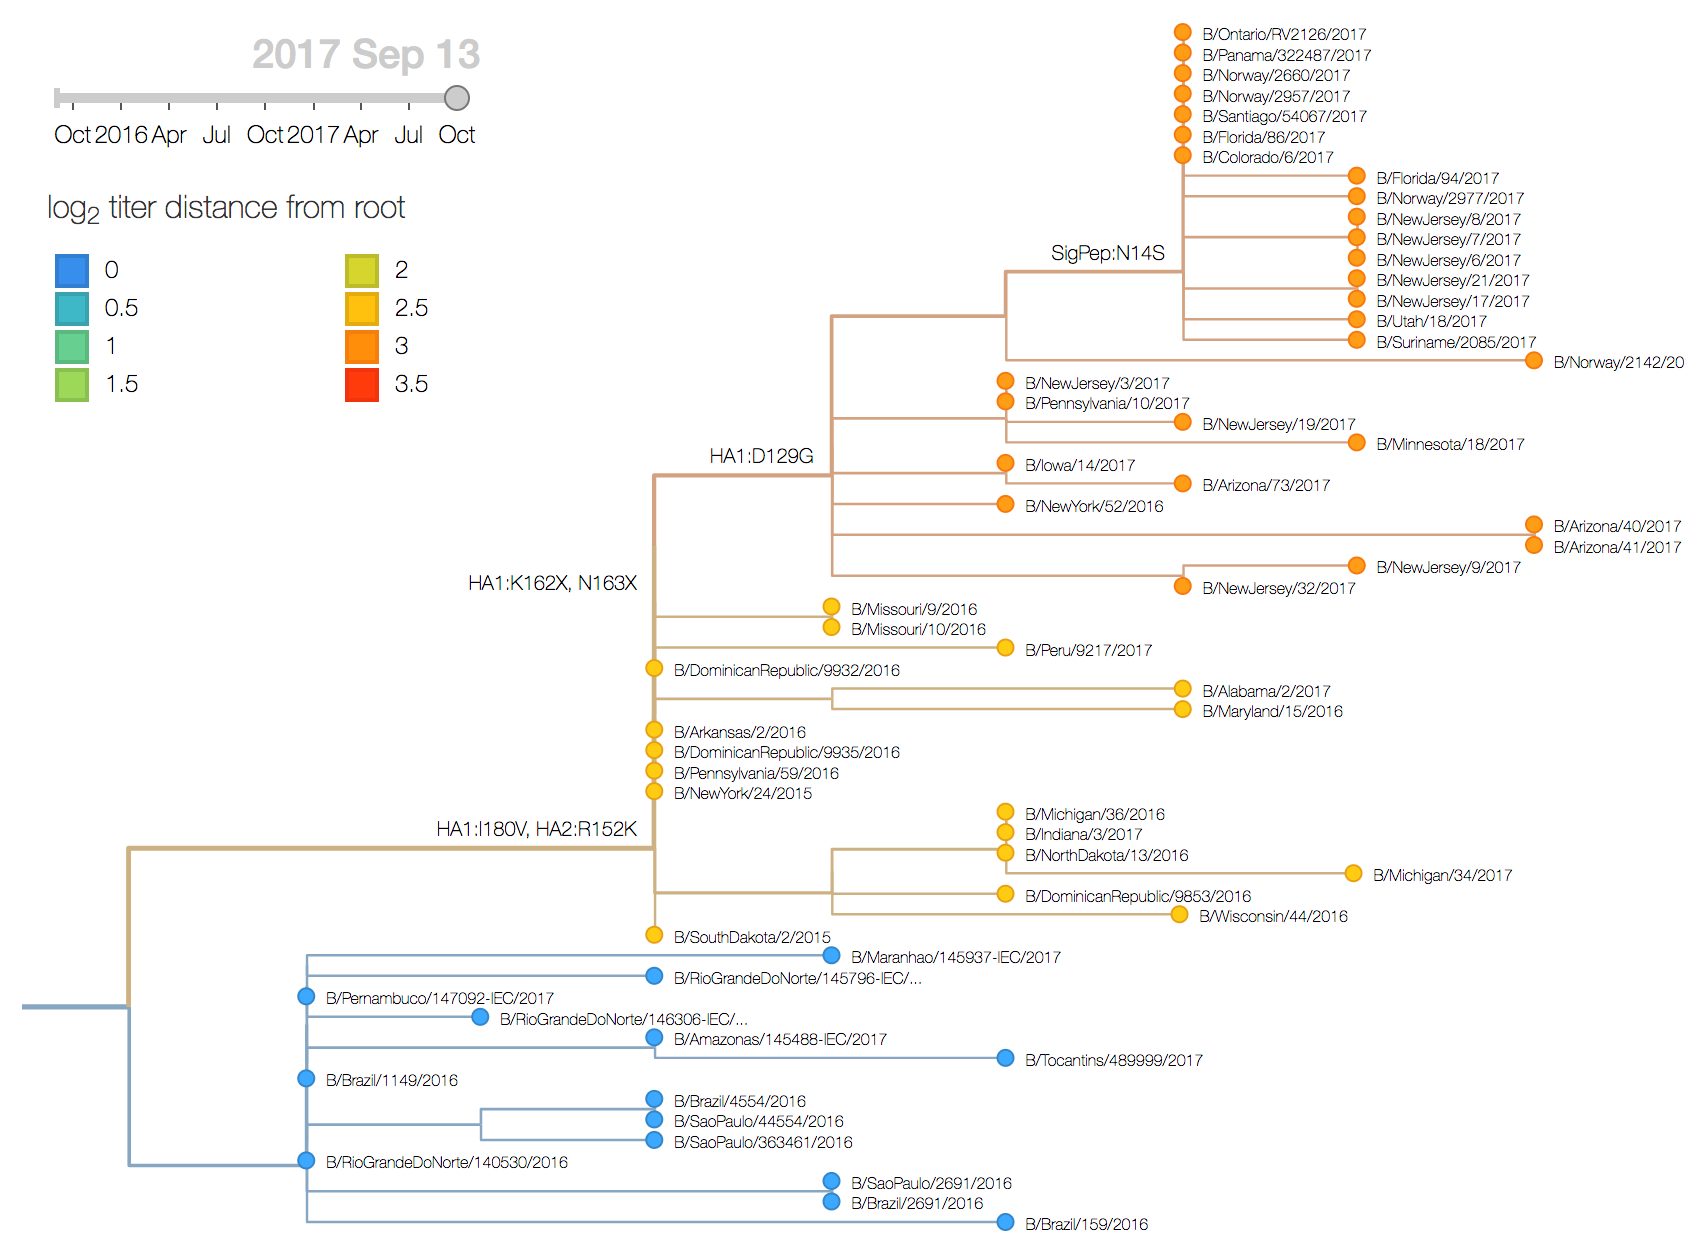
\includegraphics[width=0.95\textwidth]{../figures/sep-2017/vic_tree_titer_model.png}
  \caption{\textbf{Antigenic evolution of the B/Vic 162-/163- clade.}
  The tree model estimates a drop in HI titers by 3 units.
  }
  \label{Vic_titers}
\end{figure}

The clade bearing 129G, 162--, 163-- and 180V appears clearly drifted
according to HI measurements provided by the Influenza Division at the
US CDC, see \FIG{Vic_titers}. We estimate an approximately 8-fold titer drop (3 antigenic
units) of drift from vaccine strain B/Brisbane/60/2008. Separately, a
small number of recent viruses sampled in Hong Kong have a 9bp deletion
overlapping codons 162, 163, 164, and 165 along with a mutation I180T.
While based on limited data, the tree model estimates an 1.2 unit titer
drop.



\emph{Although the clade bearing 129G, 162--, 163-- and 180V is almost
certainly antigenically drifted, it's slow spread up to the this point
suggests that it is unlikely to predominate in a year's time. We would
advise careful monitoring as further mutations may enhance spread or
similar mutations might emerge on fitter backgrounds.}

\clearpage
\section*{B/Yam}
\addcontentsline{toc}{section}{B/Yam}

\textbf{A clade comprising M251V with clade 3 viruses continues to
dominate. The is little genetic differentiation within this clade and no
evidence of antigenic evolution.}

We base our primary analysis on a set of viruses collected between Oct
2015 and Aug 2017, comprising between 50 and 250 viruses per month
during relevant months of 2017, see \FIG{Yam_counts}. We use all available data when
estimating frequencies of mutations and weight samples appropriately by
regional population size and relative sampling intensity to arrive at a
putatively unbiased global frequency estimate. Phylogenetic analyses are
based on a representative sample of about 2000 viruses.

\begin{figure}[H]
  \centering
  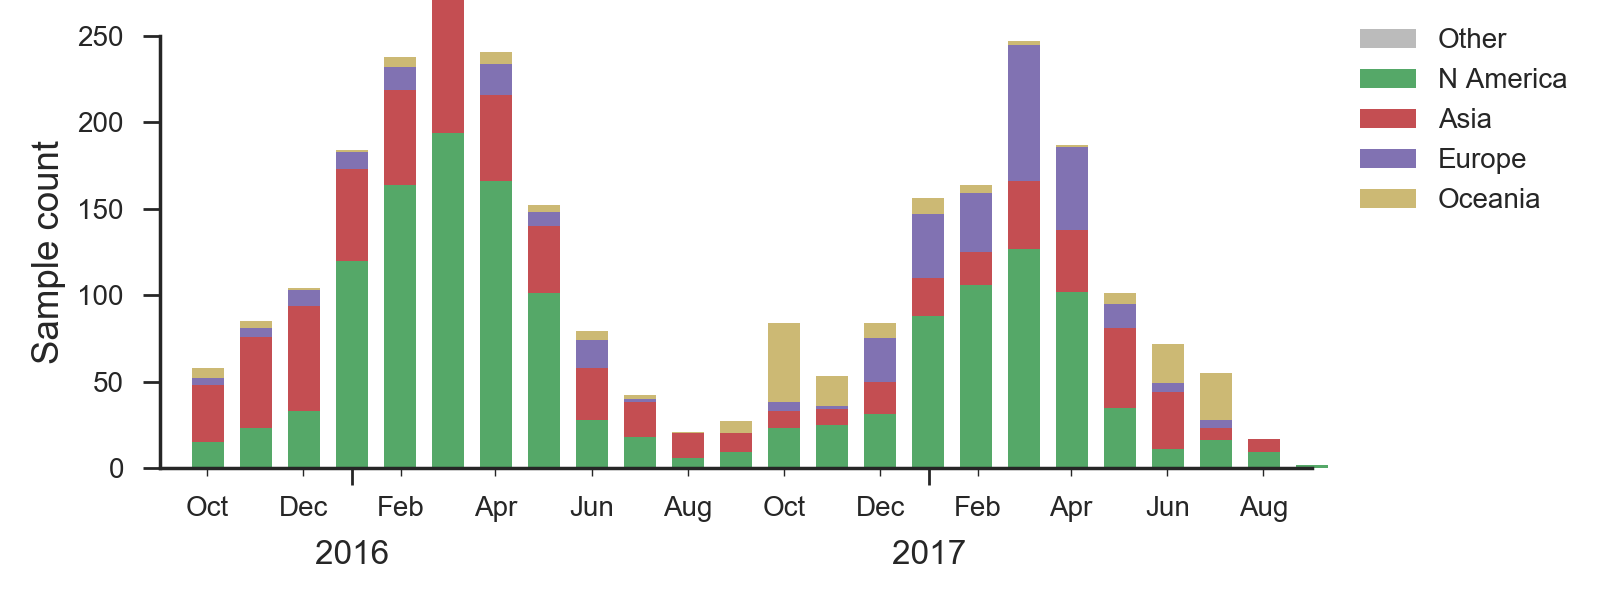
\includegraphics[width=0.95\textwidth]{../figures/sep-2017/yam_counts.png}
  \caption{\textbf{Sample counts through time and across regions.}
  This is a stacked bar plot, so that in good months there are $\sim$200 total samples.
  }
  \label{Yam_counts}
\end{figure}

\clearpage
\begin{figure}[H]
  \centering
  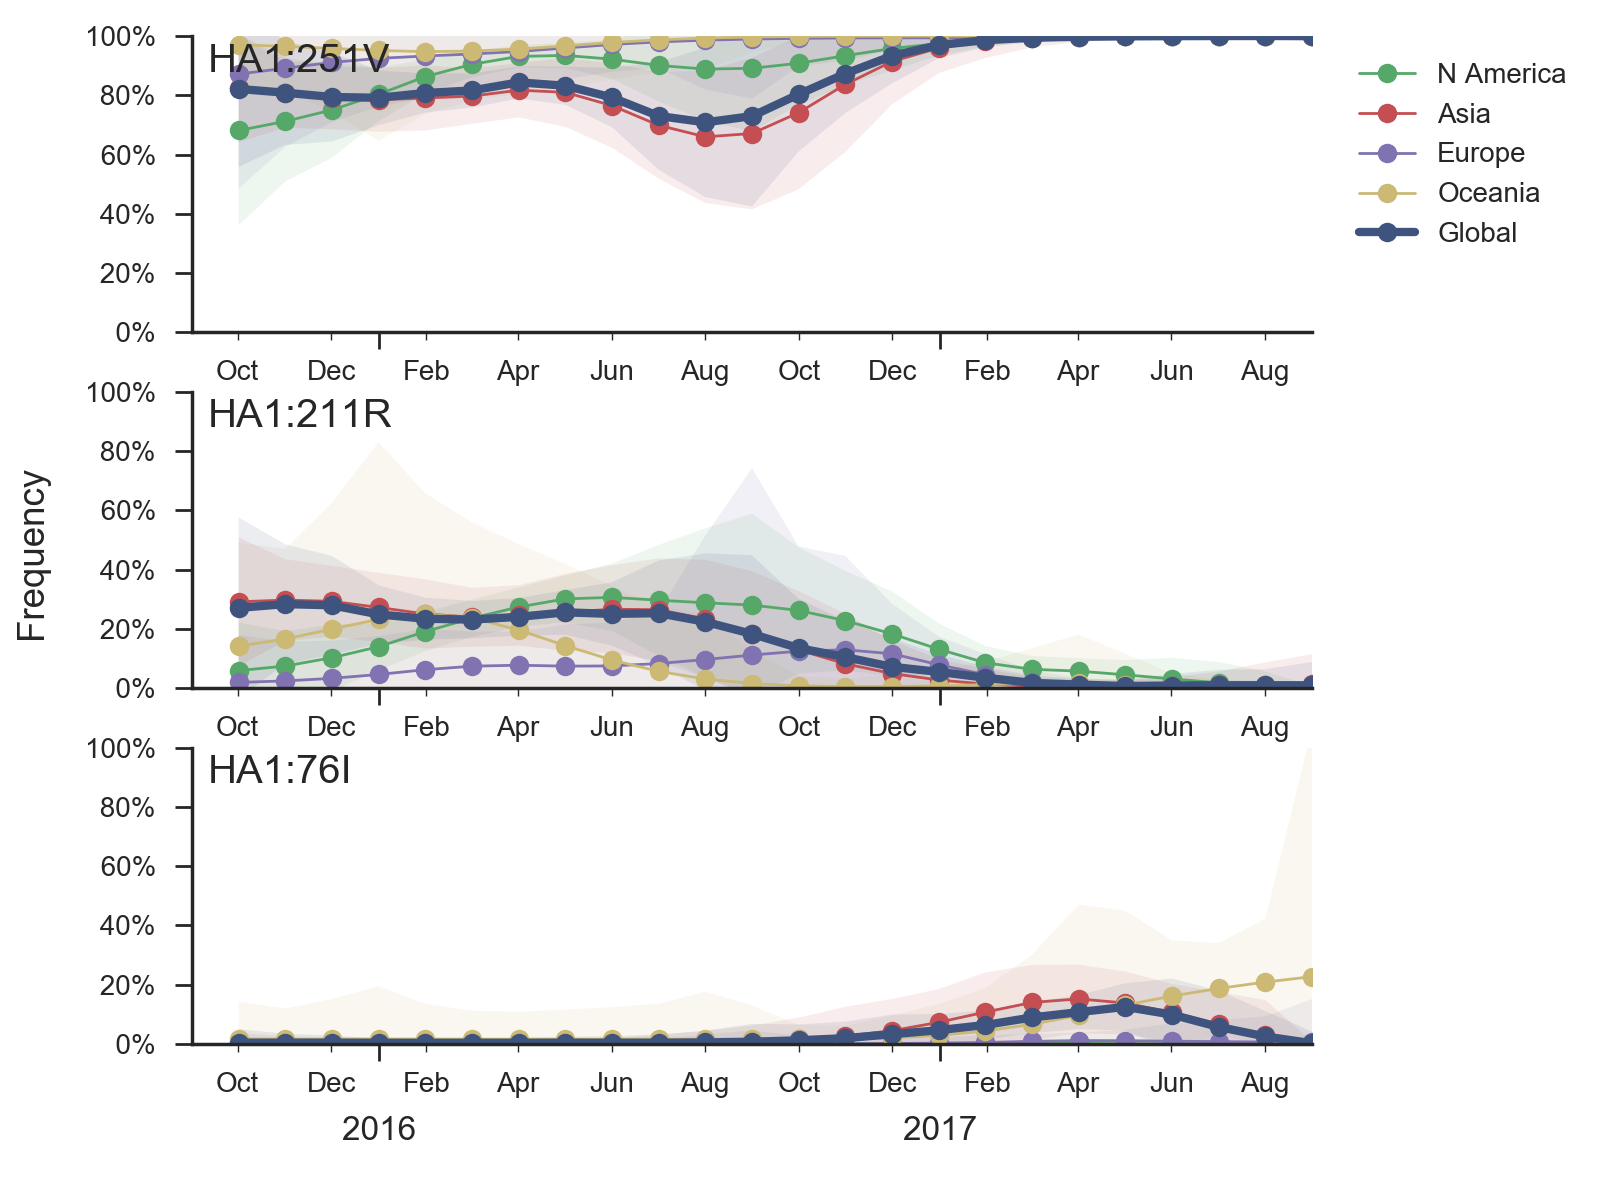
\includegraphics[width=0.95\textwidth]{../figures/sep-2017/yam_mutations.png}
  \caption{\textbf{Frequency trajectories of B/Yam variants.}
  }
  \label{Yam_mutations}
\end{figure}
Clade 2 viruses appear to be extinct from the world. Clade 3 viruses
have continued to evolve and genetic diversity relative to vaccine
strain B/Phuket/3073/2013 has emerged. Of note the clade comprising
M251V dominates the population with over 99\% frequency, see \FIG{Yam_mutations}. The subclade
within M251V comprising K211R has decreased in frequency and is now
extinct or nearly extinct. The only notable subclade with the M251V
clade is that bearing T76I that has circulated at low frequency.


\begin{figure}[H]
  \centering
  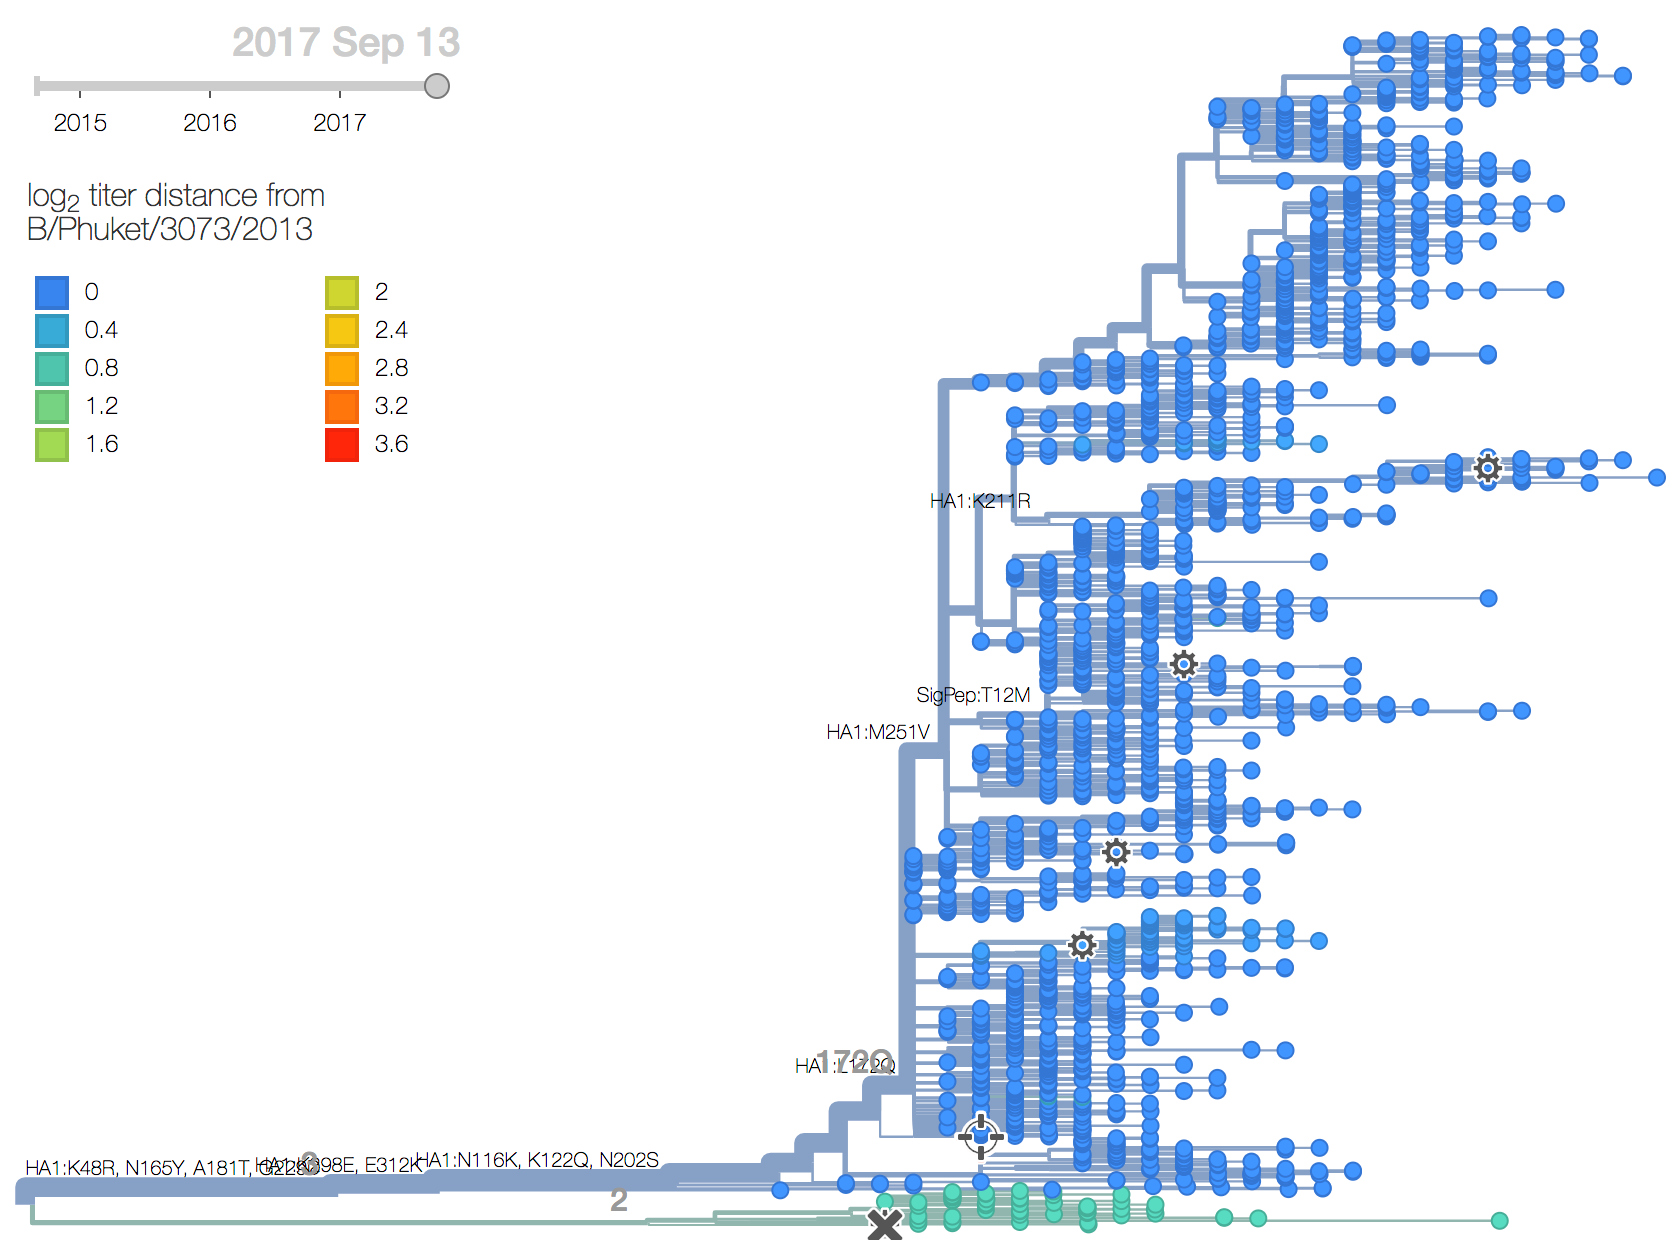
\includegraphics[width=0.8\textwidth]{../figures/sep-2017/yam_tree_titer_model.png}
  \caption{\textbf{B/Yam phylogeny colored by antigenic distance from B/Phuket/3073/2013.} The tree model of antigenic distances infers no antigenic evolution.
  }
  \label{Yam_tree}
\end{figure}

Based on HI measurements provided by the Influenza Division at the US
CDC, we find no evidence for antigenic evolution within clade 3 viruses
and the vaccine B/Phuket/3073/2013 remains well matched to circulating
viruses, see \FIG{Yam_tree}.


\emph{Barring the emergence of a new selective variant we anticipate
relative stasis of B/Yam viruses in the coming year.}

\clearpage
\pagebreak

%%% References %%%
\bibliographystyle{plos}
\bibliography{references}

\end{document}
